\section{Resultados}
\label{sec:resu}

Se simuló con Matlab\textsuperscript{\textregistered} una salida de un \emph{RO} muestreada uniformemente sin \textit{jitter} y se generó un archivo de salida con una longitud de $N_b = 7.000.000$ de bits.
Se exploró un conjunto de cien valores de relación de muestreo $r = T_s/T \in [6,5; 9,5]$ (donde $T_s$ es el período de muestreo y $T$ es el período de salida \emph{RO}).
\textit{Jitter} con una distribución normal con un conjunto de diferentes valores de varianza $\sigma_s$ (ver a continuación) se agregaron y se generaron nuevos archivos de la misma longitud.
Nuestro método emula el verdadero proceso de muestreo de la salida ruidosa de un \emph{RO} real; el código detallado se publicó en Mathworks \cite{MathworksMaxi}.

Por cada valor de $\sigma_s$, ten surrogates (each one with a different random initial condition) were generated and new files with $N_b$ bits each were stored. It was assumed that jitter of individual samples is independent, normal distributed random variables, with zero mean value and variance $\sigma_i=\sigma_s$. Consequently, the variance of the accumulated jitter over one period $T$ is given by $\sigma^2_T=r \sigma^2_s$ \cite{Valtchanov2008}. The values considered  are $\sigma_T=\{0,$ $0.001,$ $0.002,$ $0.003,$ $0.004,$ $0.005,$ $0.007,$ $0.01,$ $0.02,$ $0.02,$ $0.04,$ $0.05,$ $0.07,$ $0.1\}$.

Para cada valor de $\sigma_s$, se generaron diez surrogados (cada uno con una condición inicial aleatoria diferente) y se almacenaron nuevos archivos con $N_b$ bits cada uno. Se asumió que el \textit{jitter} de las muestras individuales es independiente, con variables aleatorias distribuidas normales y un valor medio cero y varianza $\sigma_i = \sigma_s$.
En consecuencia, la varianza del \textit{jitter} acumulada durante un período de $T$ está dada por $\sigma^2_T = r \sigma^2_s $ \cite{Valtchanov2008}.
Los valores considerados son $\sigma_T=\{0,$ $0.001,$ $0.002,$ $0.003,$ $0.004,$ $0.005,$ $0.007,$ $0.01,$ $0.02,$ $0.02,$ $0.04,$ $0.05,$ $0.07,$ $0.1\}$.

Por cada archivo se evaluaron todos los cuantificadores definidos en la sección \ref{sec:quanti} para $D\in[2,10]$ y $W\in[1,26]$..
Los detalles sobre la evaluación, las ventajas y los inconvenientes de cada cuantificador se informan en la sección \ref{sec:quanti}: ellos son $S_W$, $S^{(D)}_{BP}$, $H_{W}$, $H^{(D)}_{BP}$, $h$ and $h^*$. 
Aquí mostraremos solo los resultados más relevantes para mostrar la razón por la cual los dos últimos cuantificadores ($h$ y $h^*$) resultan los más adecuados para este problema.

\begin{itemize}
	\item En el caso de entropía normalizada $H_ {W}$, depende en gran medida de $W$.
	Además, el análisis de $H_{W}$ en función de $r$ muestra que no permite determinar un valor óptimo de la relación de muestreo $r$ (ver Fig. \ref{fig:H_W_rCS}).
	Este es un problema importante si los cuantificadores se van a usar para configuraciones experimentales.
	\item En el caso de la entropía de Bandt \& Pompe normalizada $H^{(D)}_{BP}$, también está presente una fuerte dependencia con la dimensión de emmbedding $D$.
	Nuevamente, no es fácil determinar el valor óptimo de $r$ del análisis de este parámetro en función de $r$ (ver Fig. \ref{fig:HBP_W_rSS}).
	\item Un comportamiento similar aparece en todos los otros funcionales relacionados con estas dos entropías.
	En resumen, nuestros resultados muestran que tanto $h$ y $h^*$ son independientes de cualquier parámetro arbitrario utilizado en su determinación estadística.
	Estos dos cuantificadores también se han considerado en dos excelentes artículos \cite{Amigo2006, Ebeling2001}.
\end{itemize}

%
\begin{figure}
\center
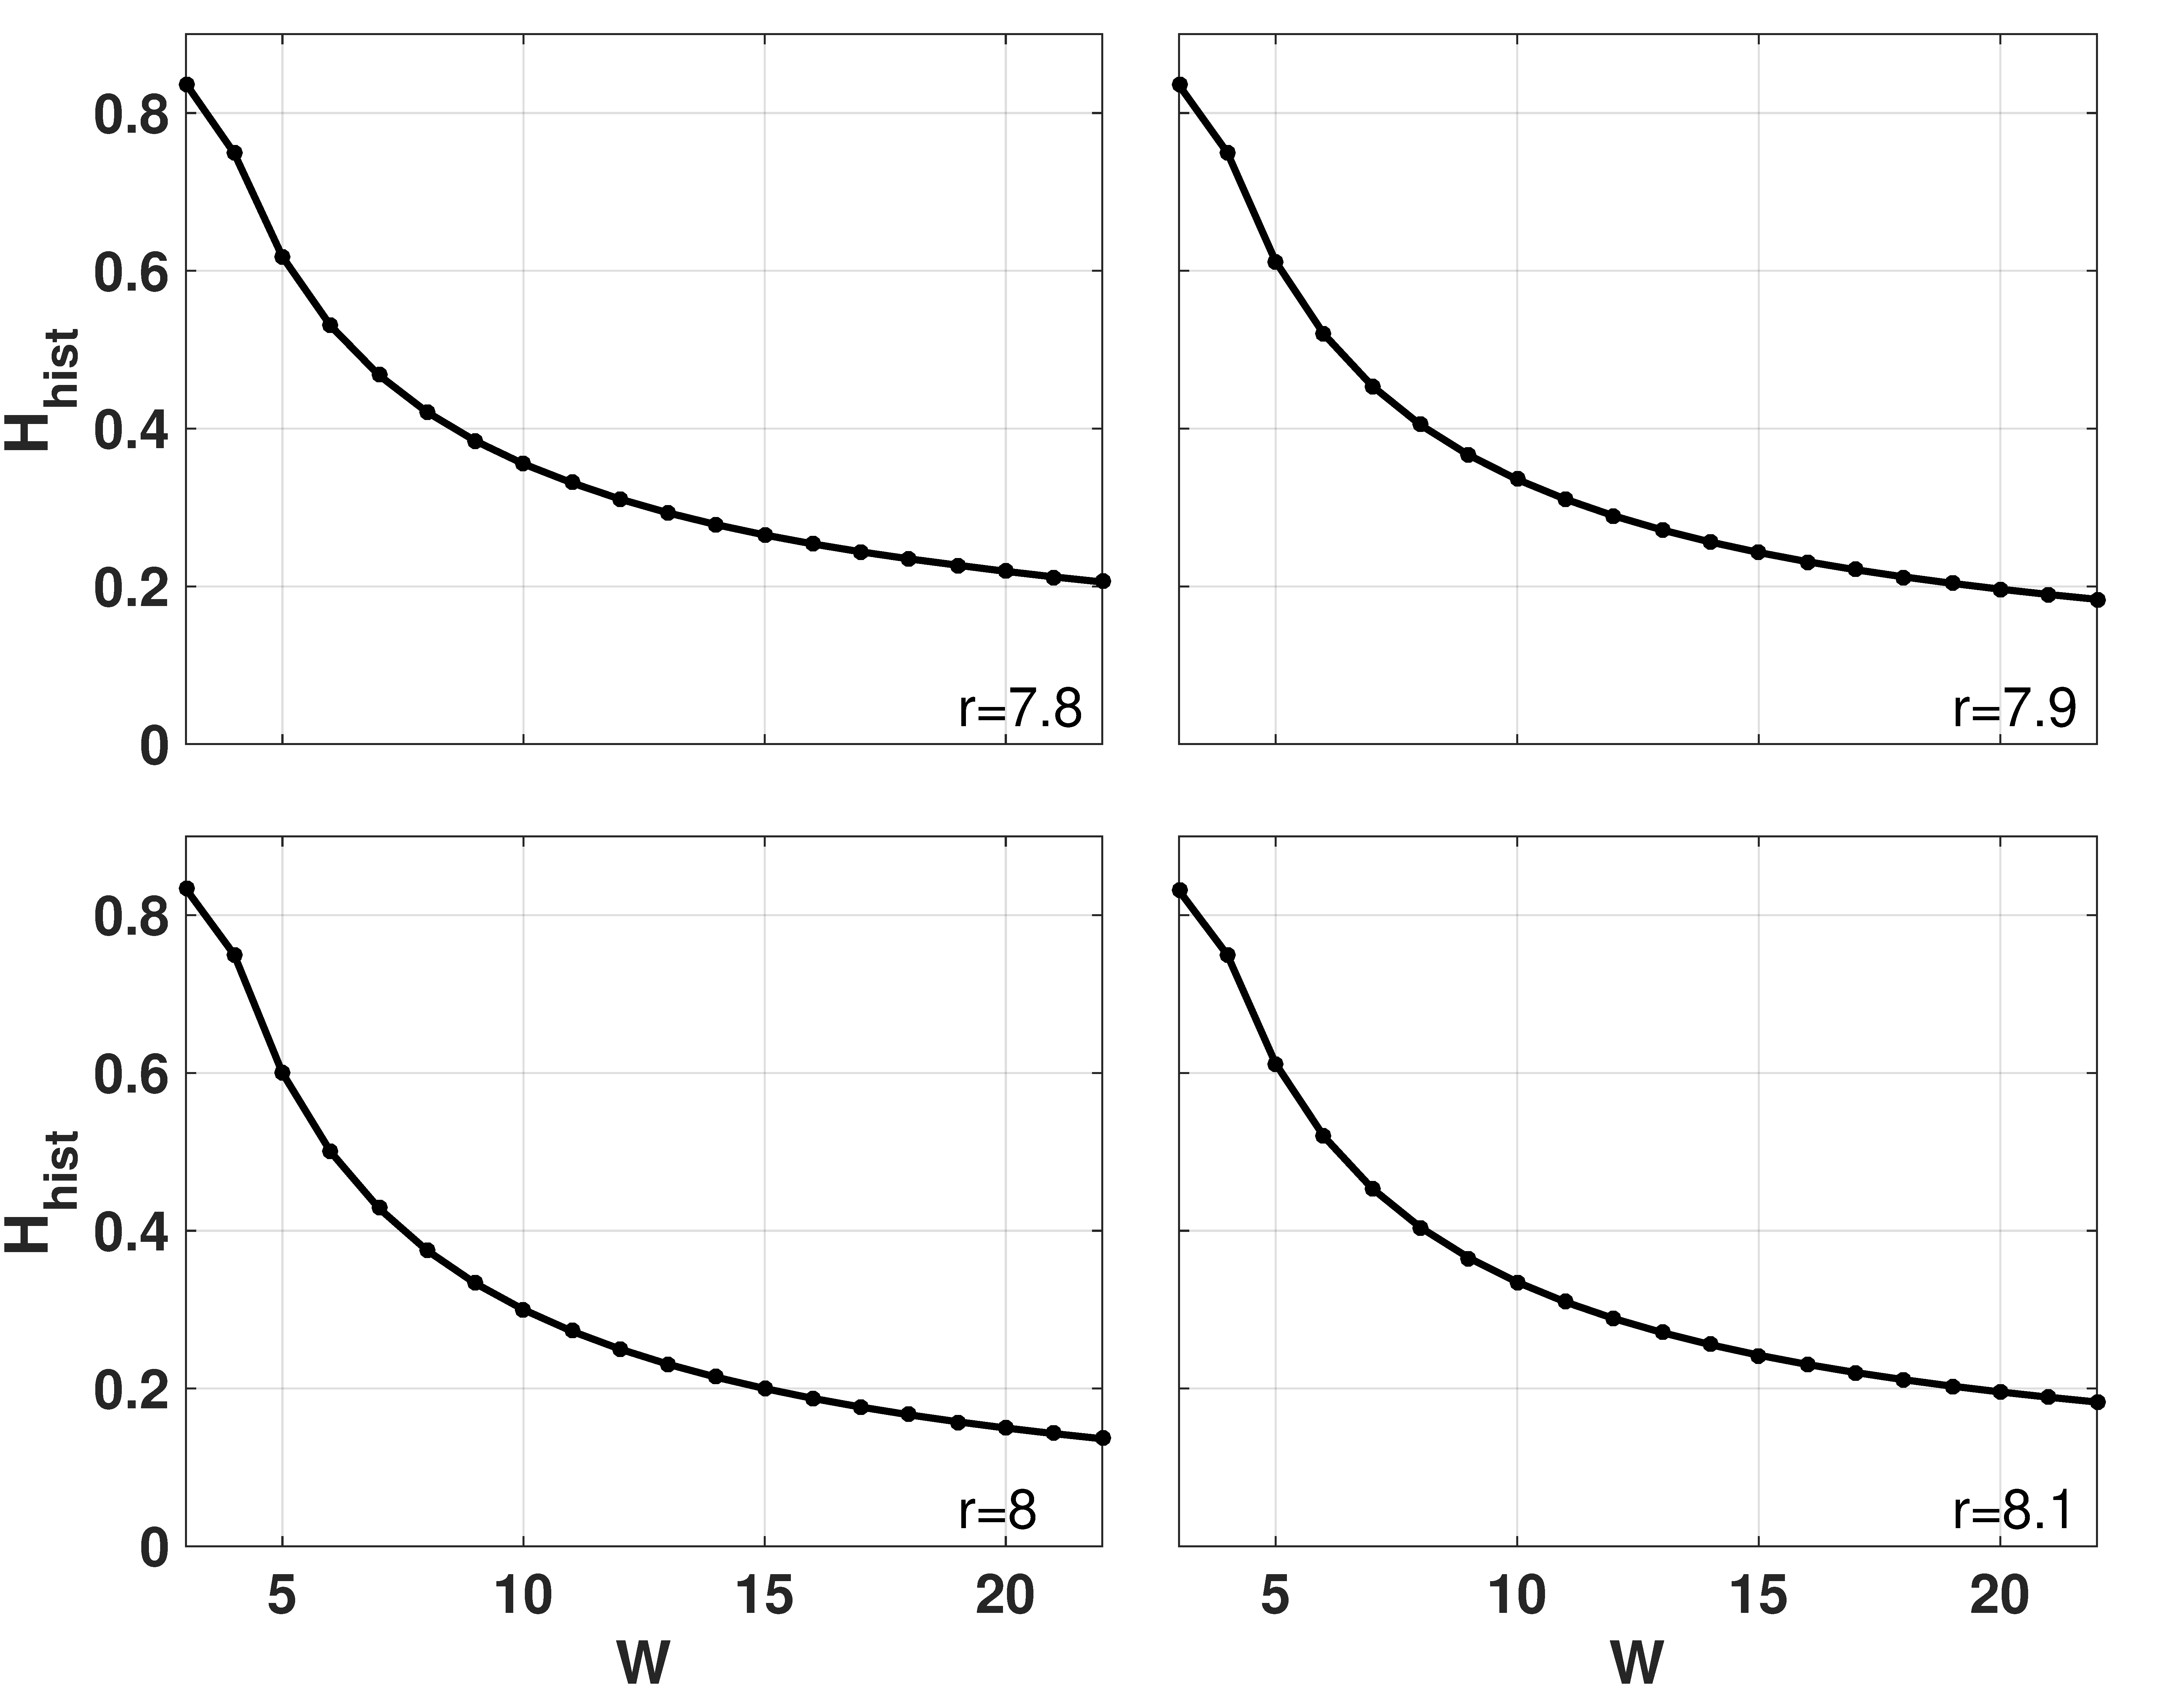
\includegraphics[width=0.8\textwidth]{H_W_rCS}
\caption{Entropía normalizada $H_W$ en función de $W$ para un \emph{RO} sin \textit{jitter} muestreado con diferentes valores de $r$.}
\label{fig:H_W_rCS}
\end{figure}
%
\begin{figure}
\center
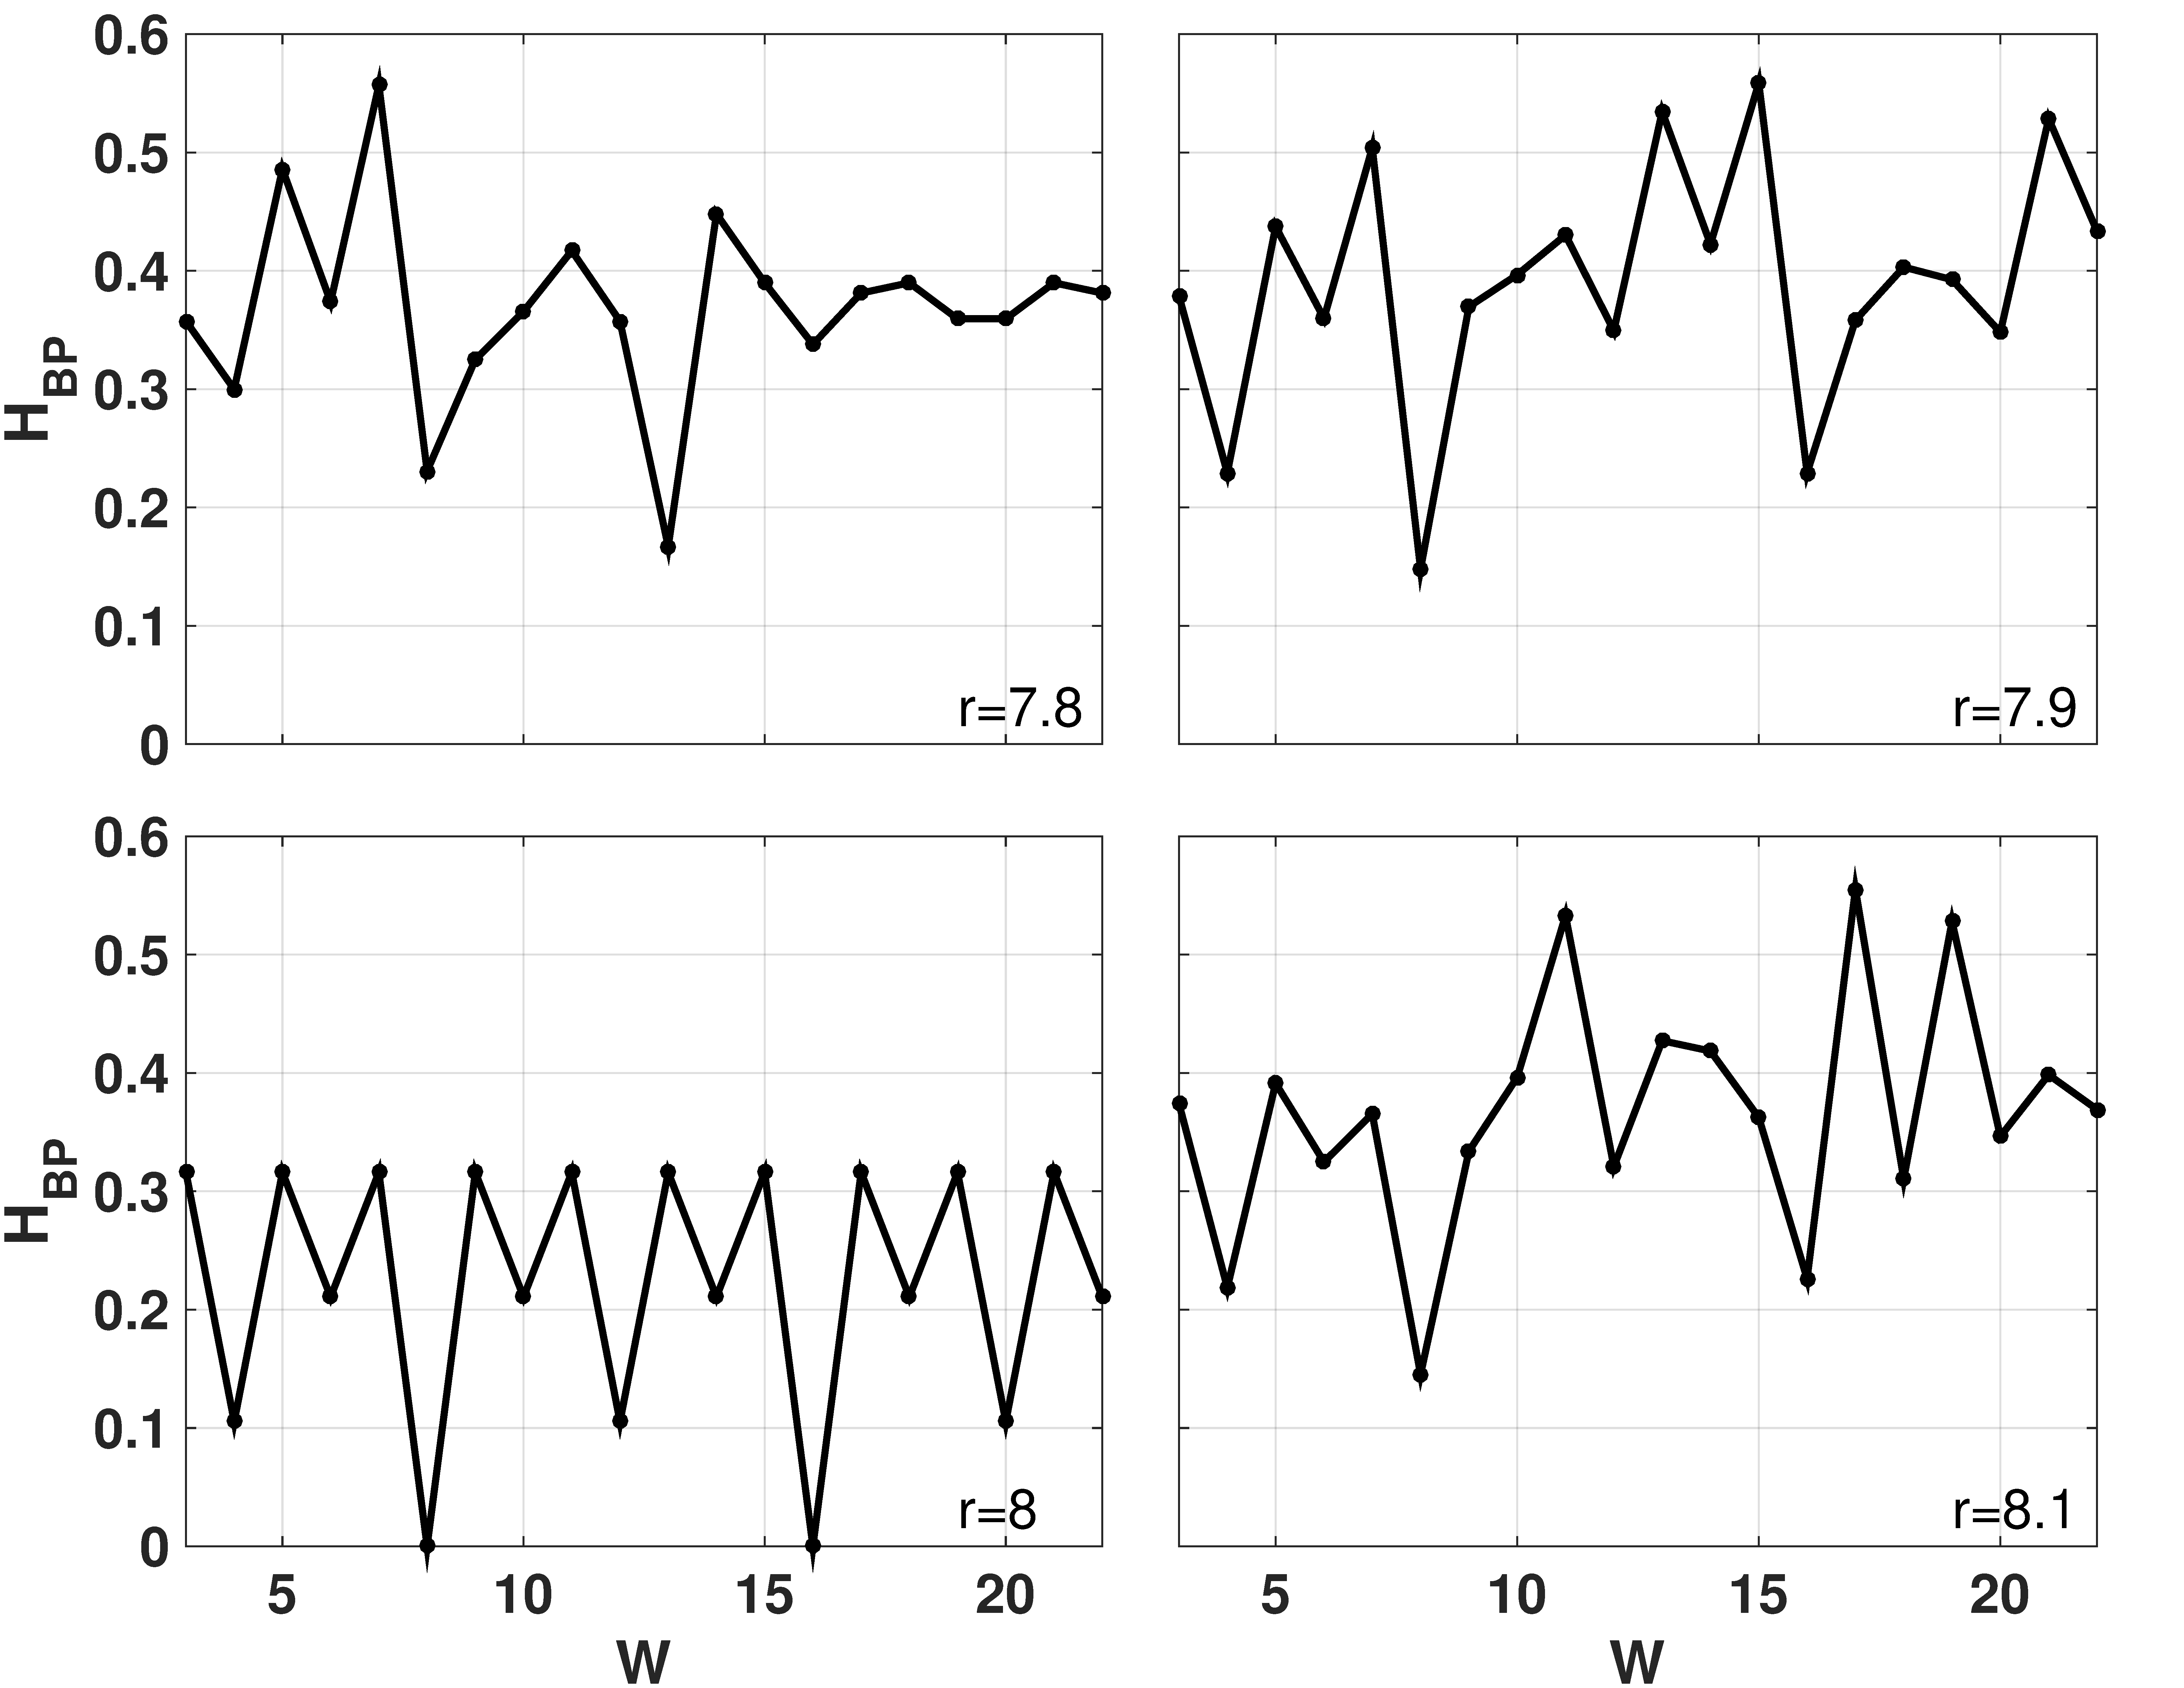
\includegraphics[ width=0.8\textwidth]{HBP_W_rSS}
\caption{$H^{(D)}_{BP}$ en función de  $W$ para un \emph{RO} sin \textit{jitter} muestreado con diferentes valores de $r$. Los cálculos fueron hechos con superposición de palabras}
\label{fig:HBP_W_rSS}
\end{figure}

Estos resultados muestran que los dos cuantificadores, $h$ y $h^*$, son apropiados para ser usados como medidores de \textit{jitter} debido a que: 
\begin{itemize} 
\item (a) Para $\sigma_T=0$ (salida sin \textit{jitter}) se acercan rápidamente a un valor limite constante ya que tanto $D$ como $W$ tienden a $\infty$ y este valor es independiente de $D$ y $W$; 
\item (b) Son funciones monótonas y proporcionales de $\sigma_T$.
\item (c) A partir de su análisis, es posible detectar el valor óptimo de la relación de muestreo $r$.
En las siguientes figuras mostraremos estas afirmaciones que son representativas de todos nuestros resultados.
\end{itemize}
%
La figura \ref{fig:hm_D_SJ} muestra la entropía diferencial de Bandt \& Pompe $h^*$, como función de $D$, con $W$ como parámetro, para un \textit{RO} sin \textit{jitter}.
Se puede ver que existe un valor umbral $W = 4$ sobre el cual todas las curvas colapsan en una sin importar el valor de $D$.
Además, la Fig. \ref{fig:hm_D_SJ} también muestra que para $D \ge 8$ todas las curvas colapsan en una, independientemente del valor de $W$.
En conclusión, si $D \ge 8$ y $W \ge 4$ obtenemos un cuantificador independiente de $D$ y $W$.
La influencia del \textit{jitter} en este cuantificador se muestra en la figura \ref{fig: hm_D_CJ}, donde $h^*$ se representa como una función de $D$ con $\sigma_T$ como parámetro.
Los valores considerados son $\sigma_T=\{0 (sin~jitter),$ $0.001,$ $0.002,$ $0.003,$ $0.004,$ $0.005,$ $0.007,$ $0.01,$ $0.02,$ $0.02,$ $0.04,$ $0.05,$ $0.07,$ $0.1\}$.
El recuadro de la Fig. \ref{fig:hm_D_CJ} muestra $h^*$ como una función de $\sigma_T$ para $D = 8$.
Este recuadro muestra que este cuantificador es una función monótona creciente de $\sigma_T$.
Finalmente, la Fig.\ref{fig: hm_r_CJ} muestra $h^*$ como una función de la relación de muestreo $r$.
En esta figura, se muestra que hay un mínimo para el $r$ correcto (en este caso $r = 8$).
Además, la sensibilidad de $h^*$ en función del \textit{jitter} es máxima para este mismo valor ideal de $r$.

\begin{figure}
\center
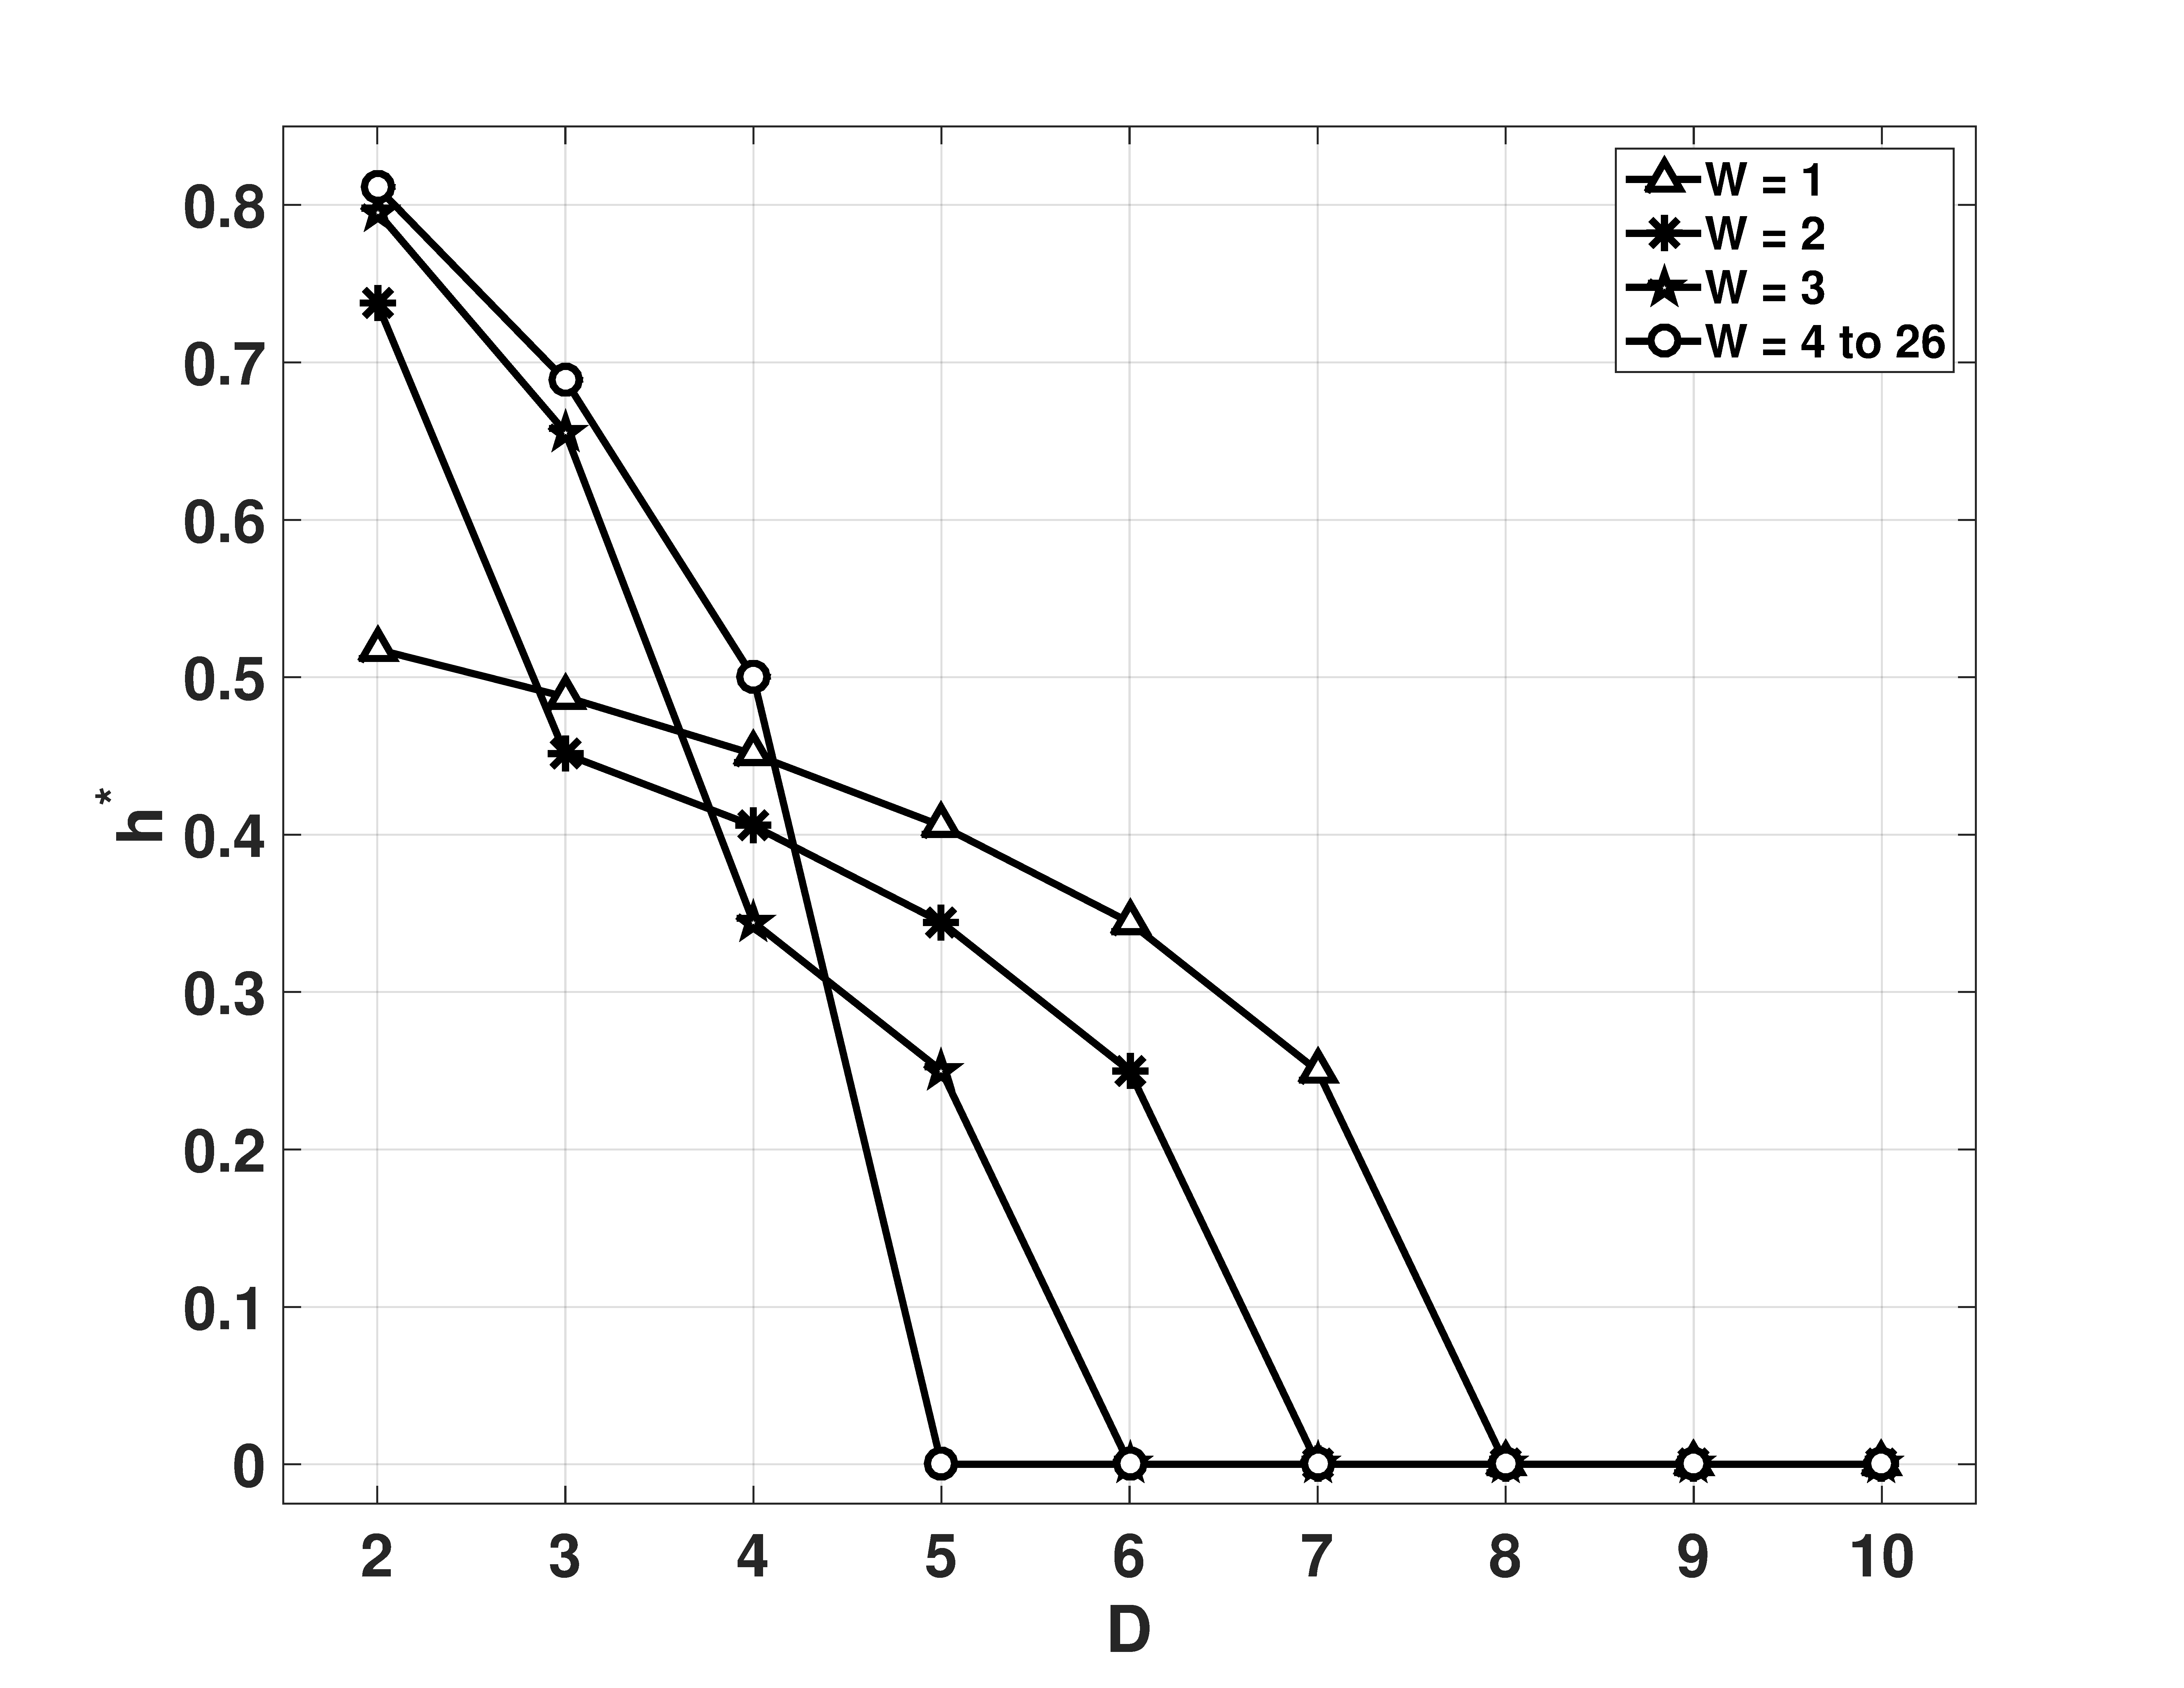
\includegraphics[ width=0.8\textwidth]{hm_D_SJ}
\caption{$h^*$ en función de $D$ para un \emph{RO} sin \textit{jitter} muestreado con $r=8$.}
\label{fig:hm_D_SJ}
\end{figure}

\begin{figure}
\center
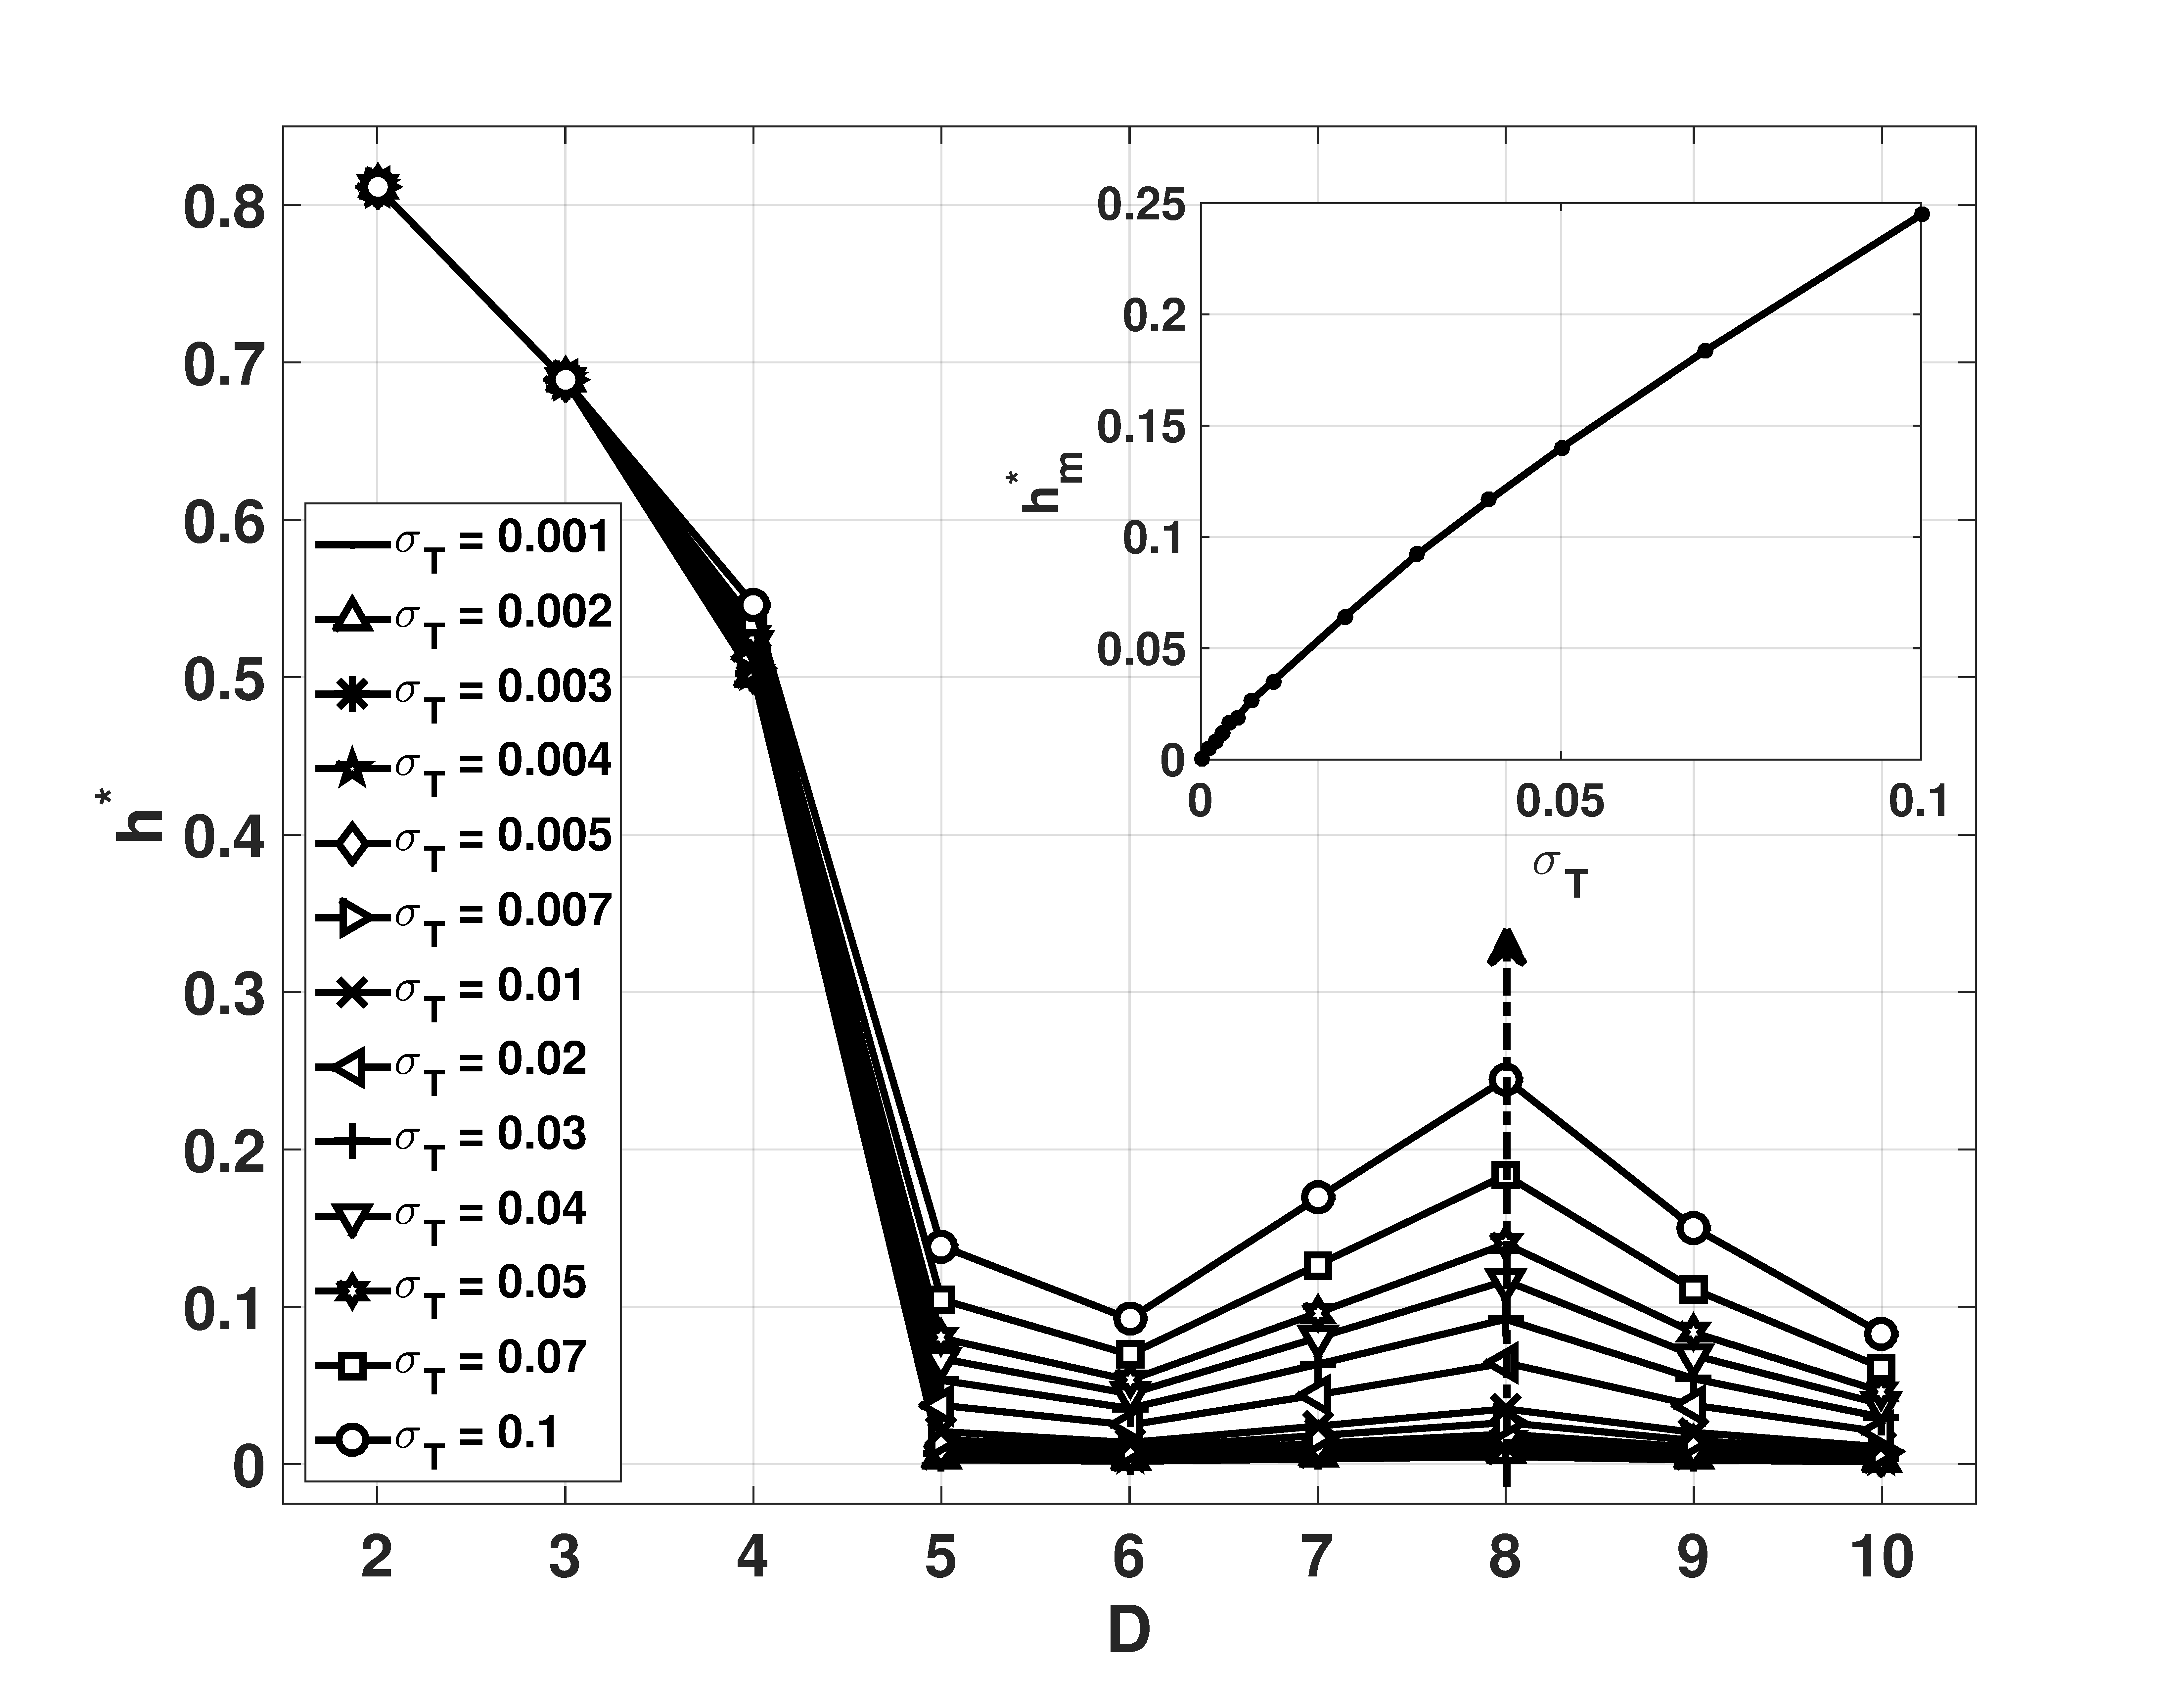
\includegraphics[width=0.8\textwidth]{hm_D_CJ}
\caption{$h^*$ en función de $D$ para un \emph{RO} muestreado con $r=8$ con longitud de palabra $W=6$ para \textit{jitter} con diferentes varianzas. El recuadro muestra $h^*$ en función de $\sigma_T$ para $r=8$, $W=6$ y $D=8$.}
\label{fig:hm_D_CJ}
\end{figure}

\begin{figure}
\center
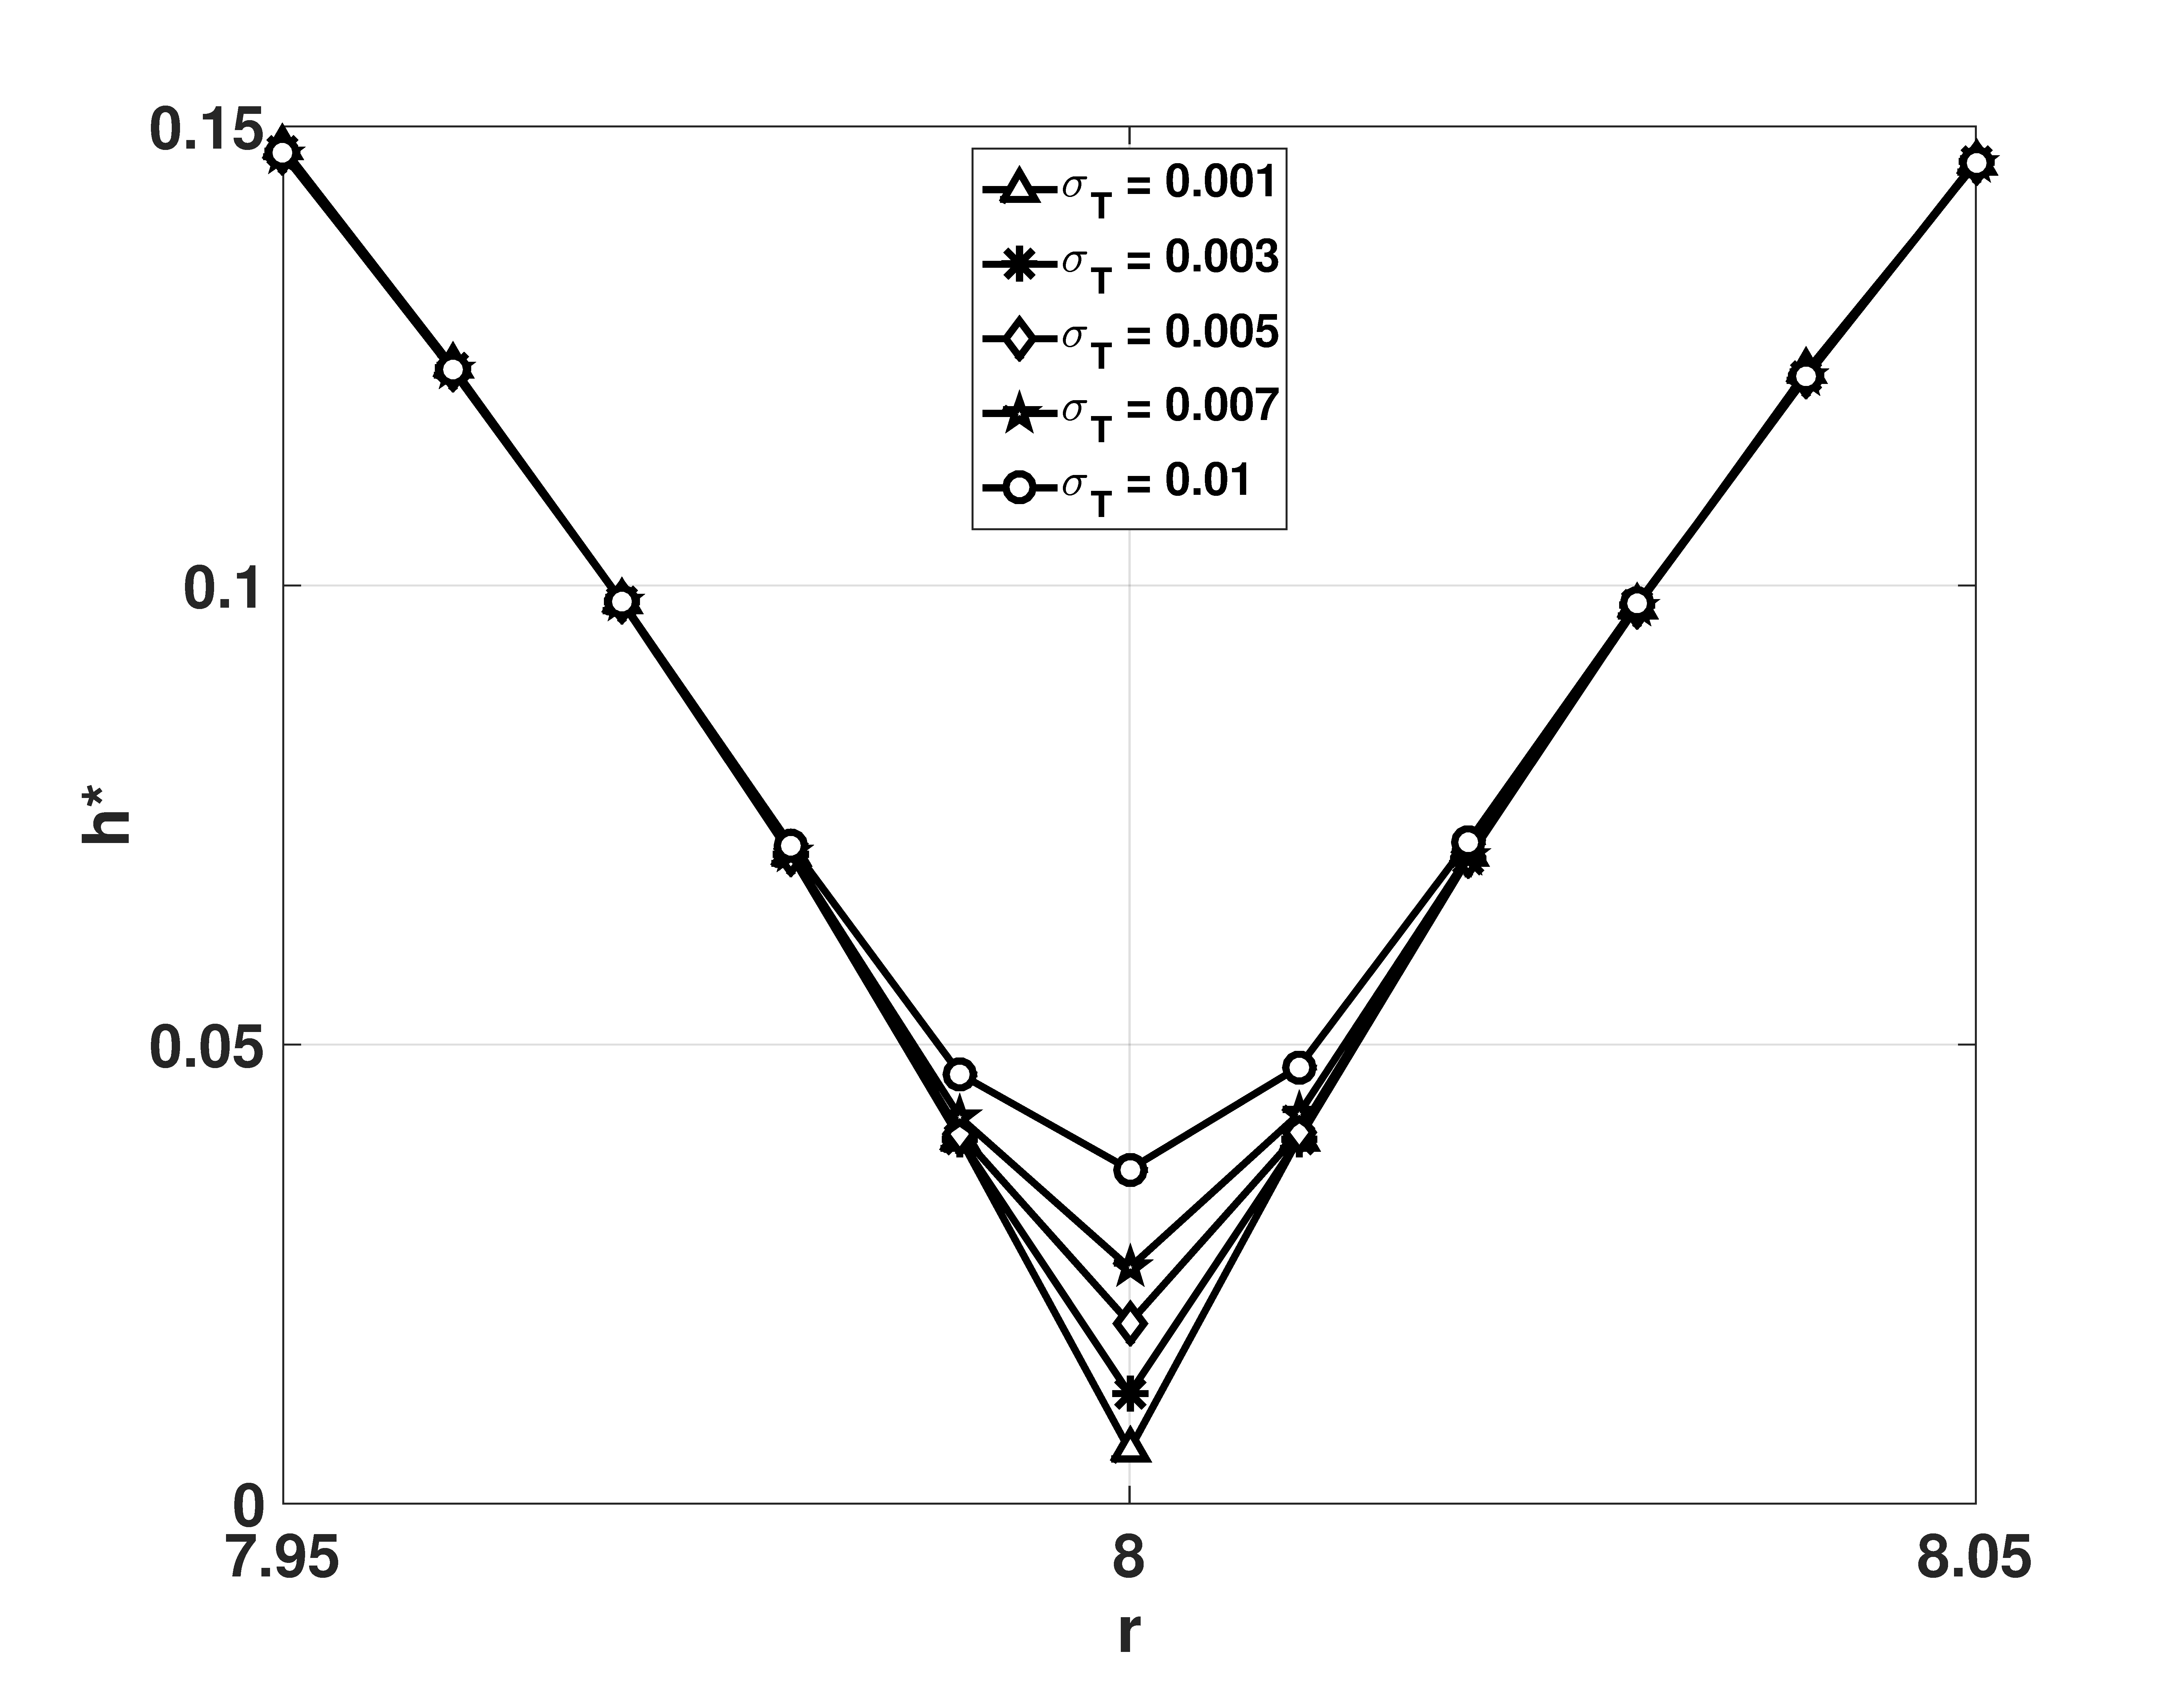
\includegraphics[ width=0.8\textwidth]{hm_r_CJ}
\caption{$h^*$ en función de $r$ para $r\in[7.95,8.05]$, con algunos $\sigma_T$, $W=6$ y $D=8$. La curva tiene un mínimo en el valor correcto de $r=8$.}
\label{fig:hm_r_CJ}
\end{figure}

Analicemos ahora el segundo cuantificador, $h$.
Este cuantificador solo depende de $W$ porque $ D $ no se usa para definir la \emph{PDF} asignada a la serie de datos.
La Fig. \ref{fig: h_W_SJ} muestra un caso sin \textit{jitter}, $h$ es independiente de $W$ para $W \ge 4$.
Para lo siguiente adoptamos $W = 6$.
La figura \ref{fig: h_W_CJ} muestra la influencia del \textit{jitter} sobre este cuantificador.
Queda claro en el recuadro de esta figura que, para el valor seleccionado $W = 6$, $h$ es una función monótona creciente de la varianza del \textit{jitter} $\sigma_T$.
La Fig. \ref{fig: h_r_CJ} muestra que $h$ tiene un mínimo cuando $r$ toma su valor óptimo ($r = 8$).
Note que este mínimo es robusto también en presencia de jitter.

\begin{figure}
\center
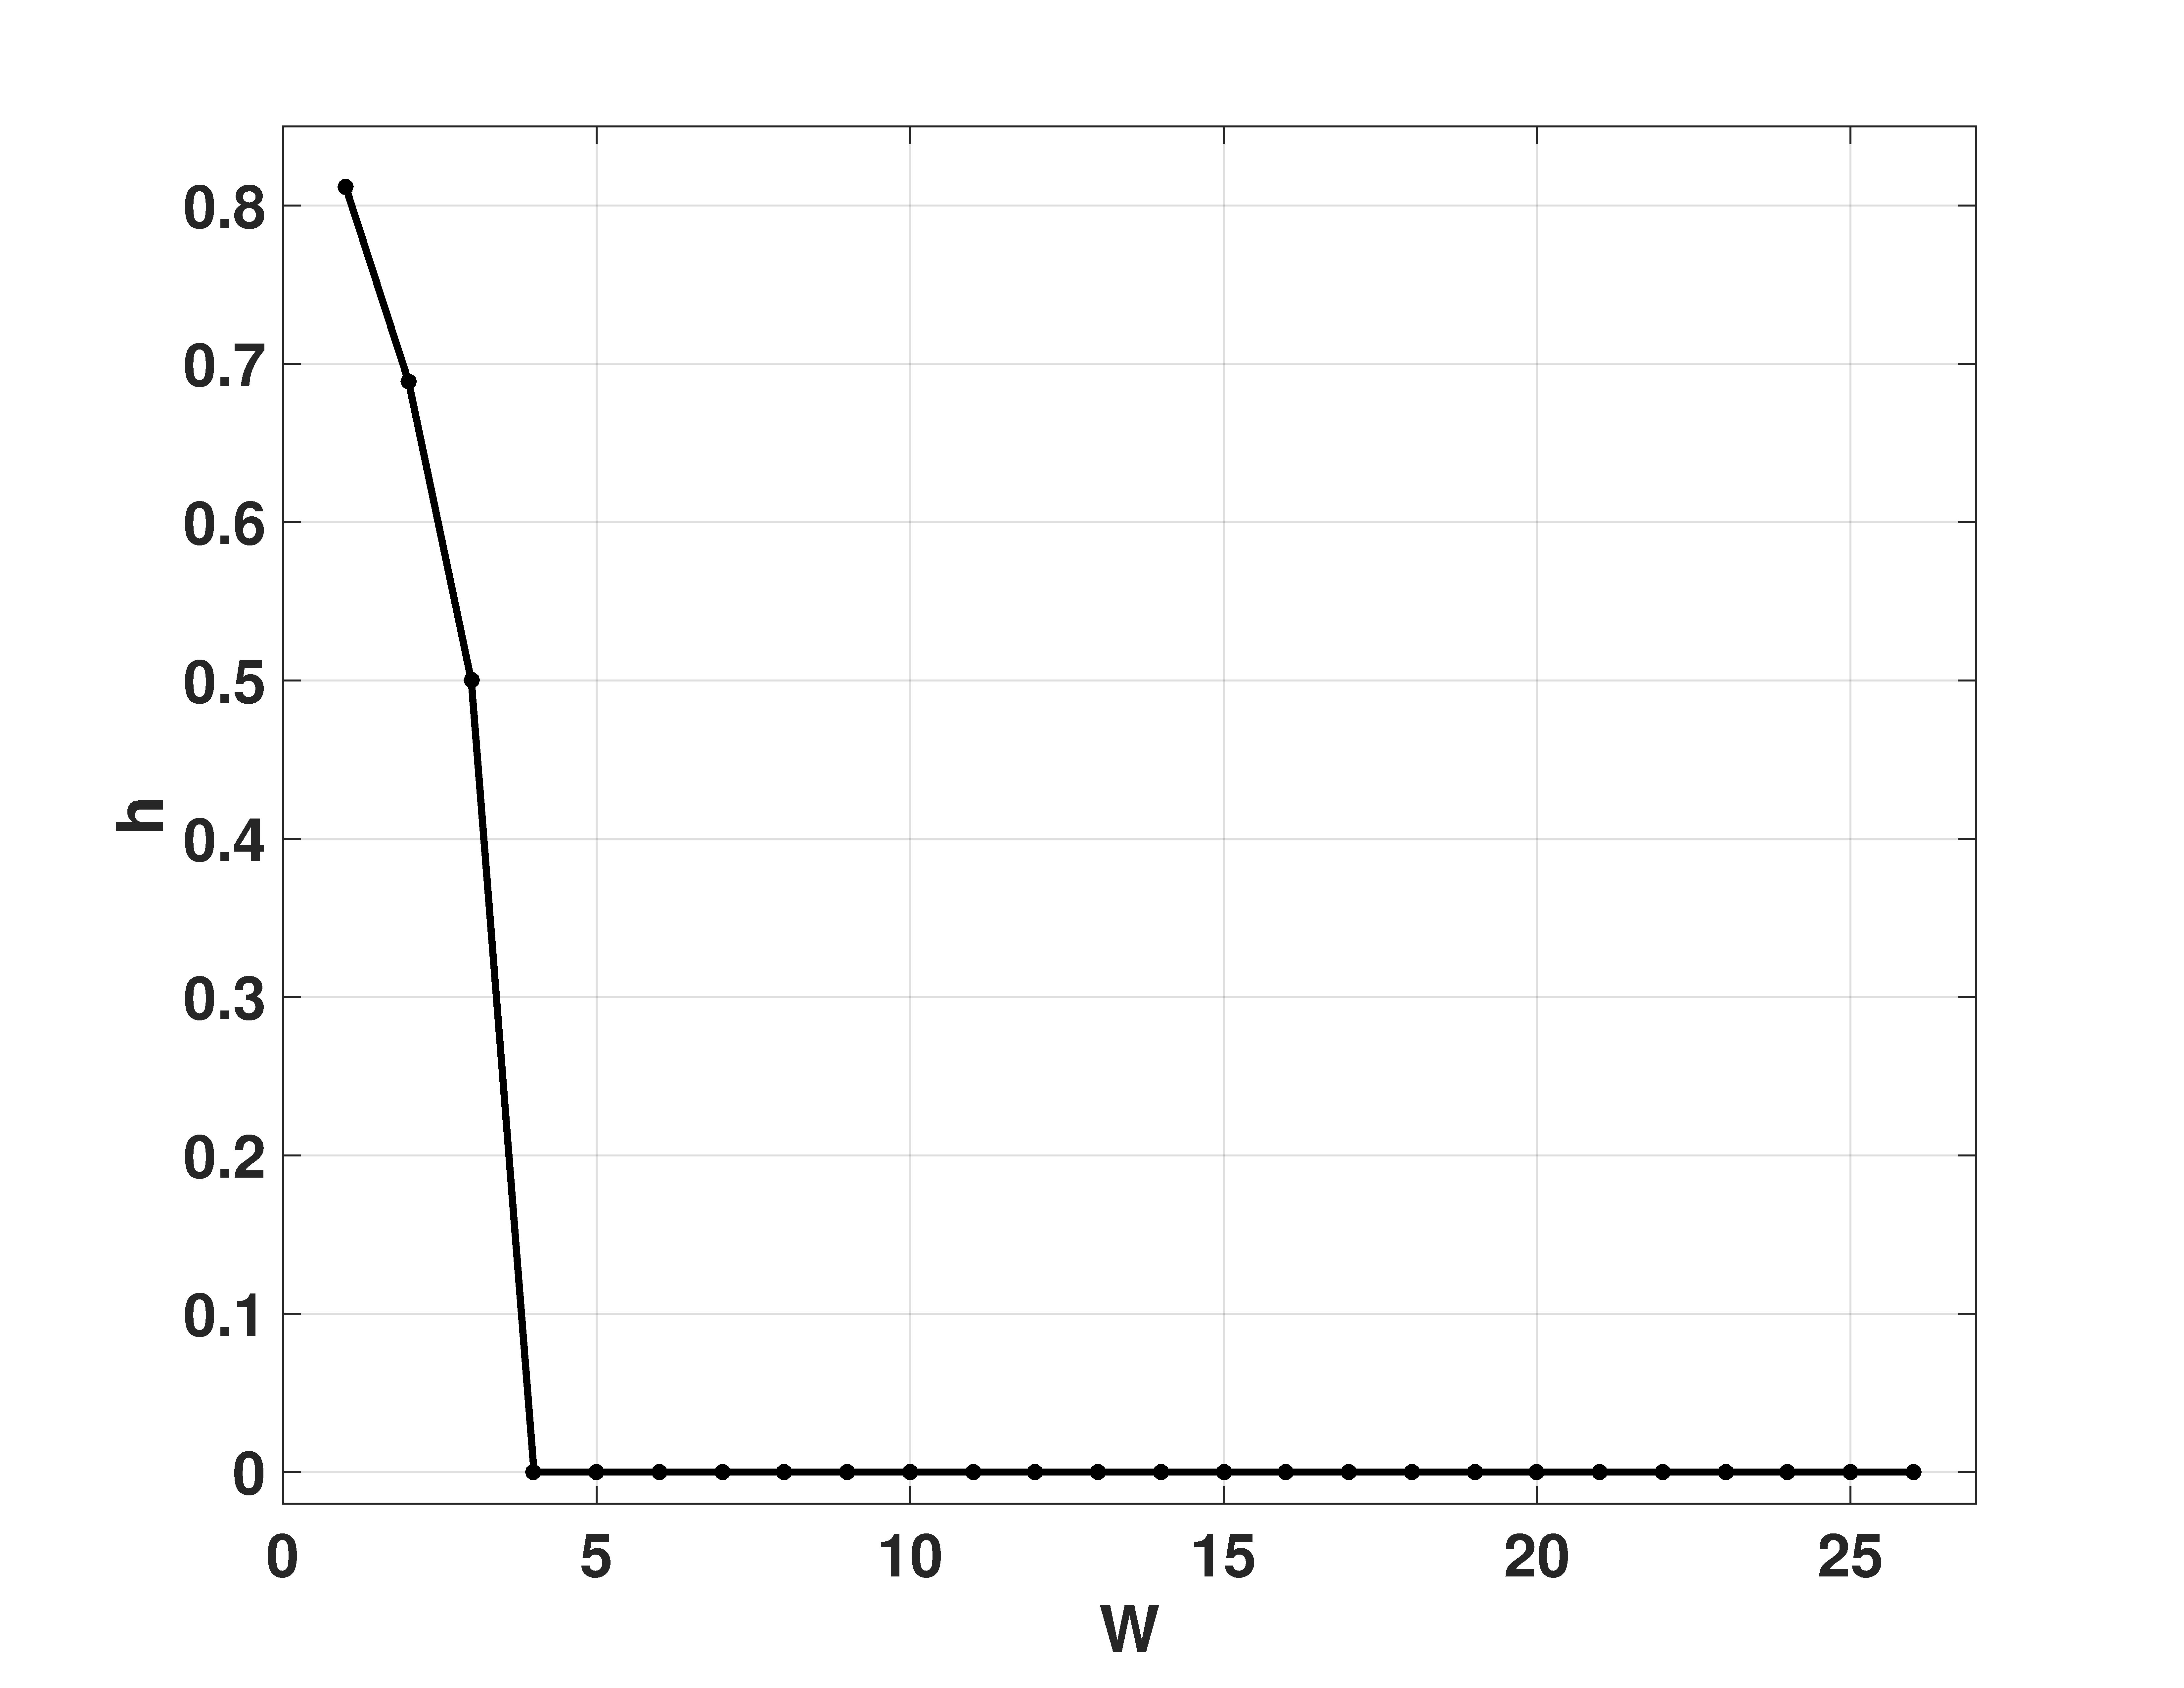
\includegraphics[width=0.8\textwidth]{h_W_SJ}
\caption{$h$ en función de $W$ para un \emph{RO} sin \textit{jitter} muestreado con $r=8$.}
\label{fig:h_W_SJ}
\end{figure}

\begin{figure}
\center
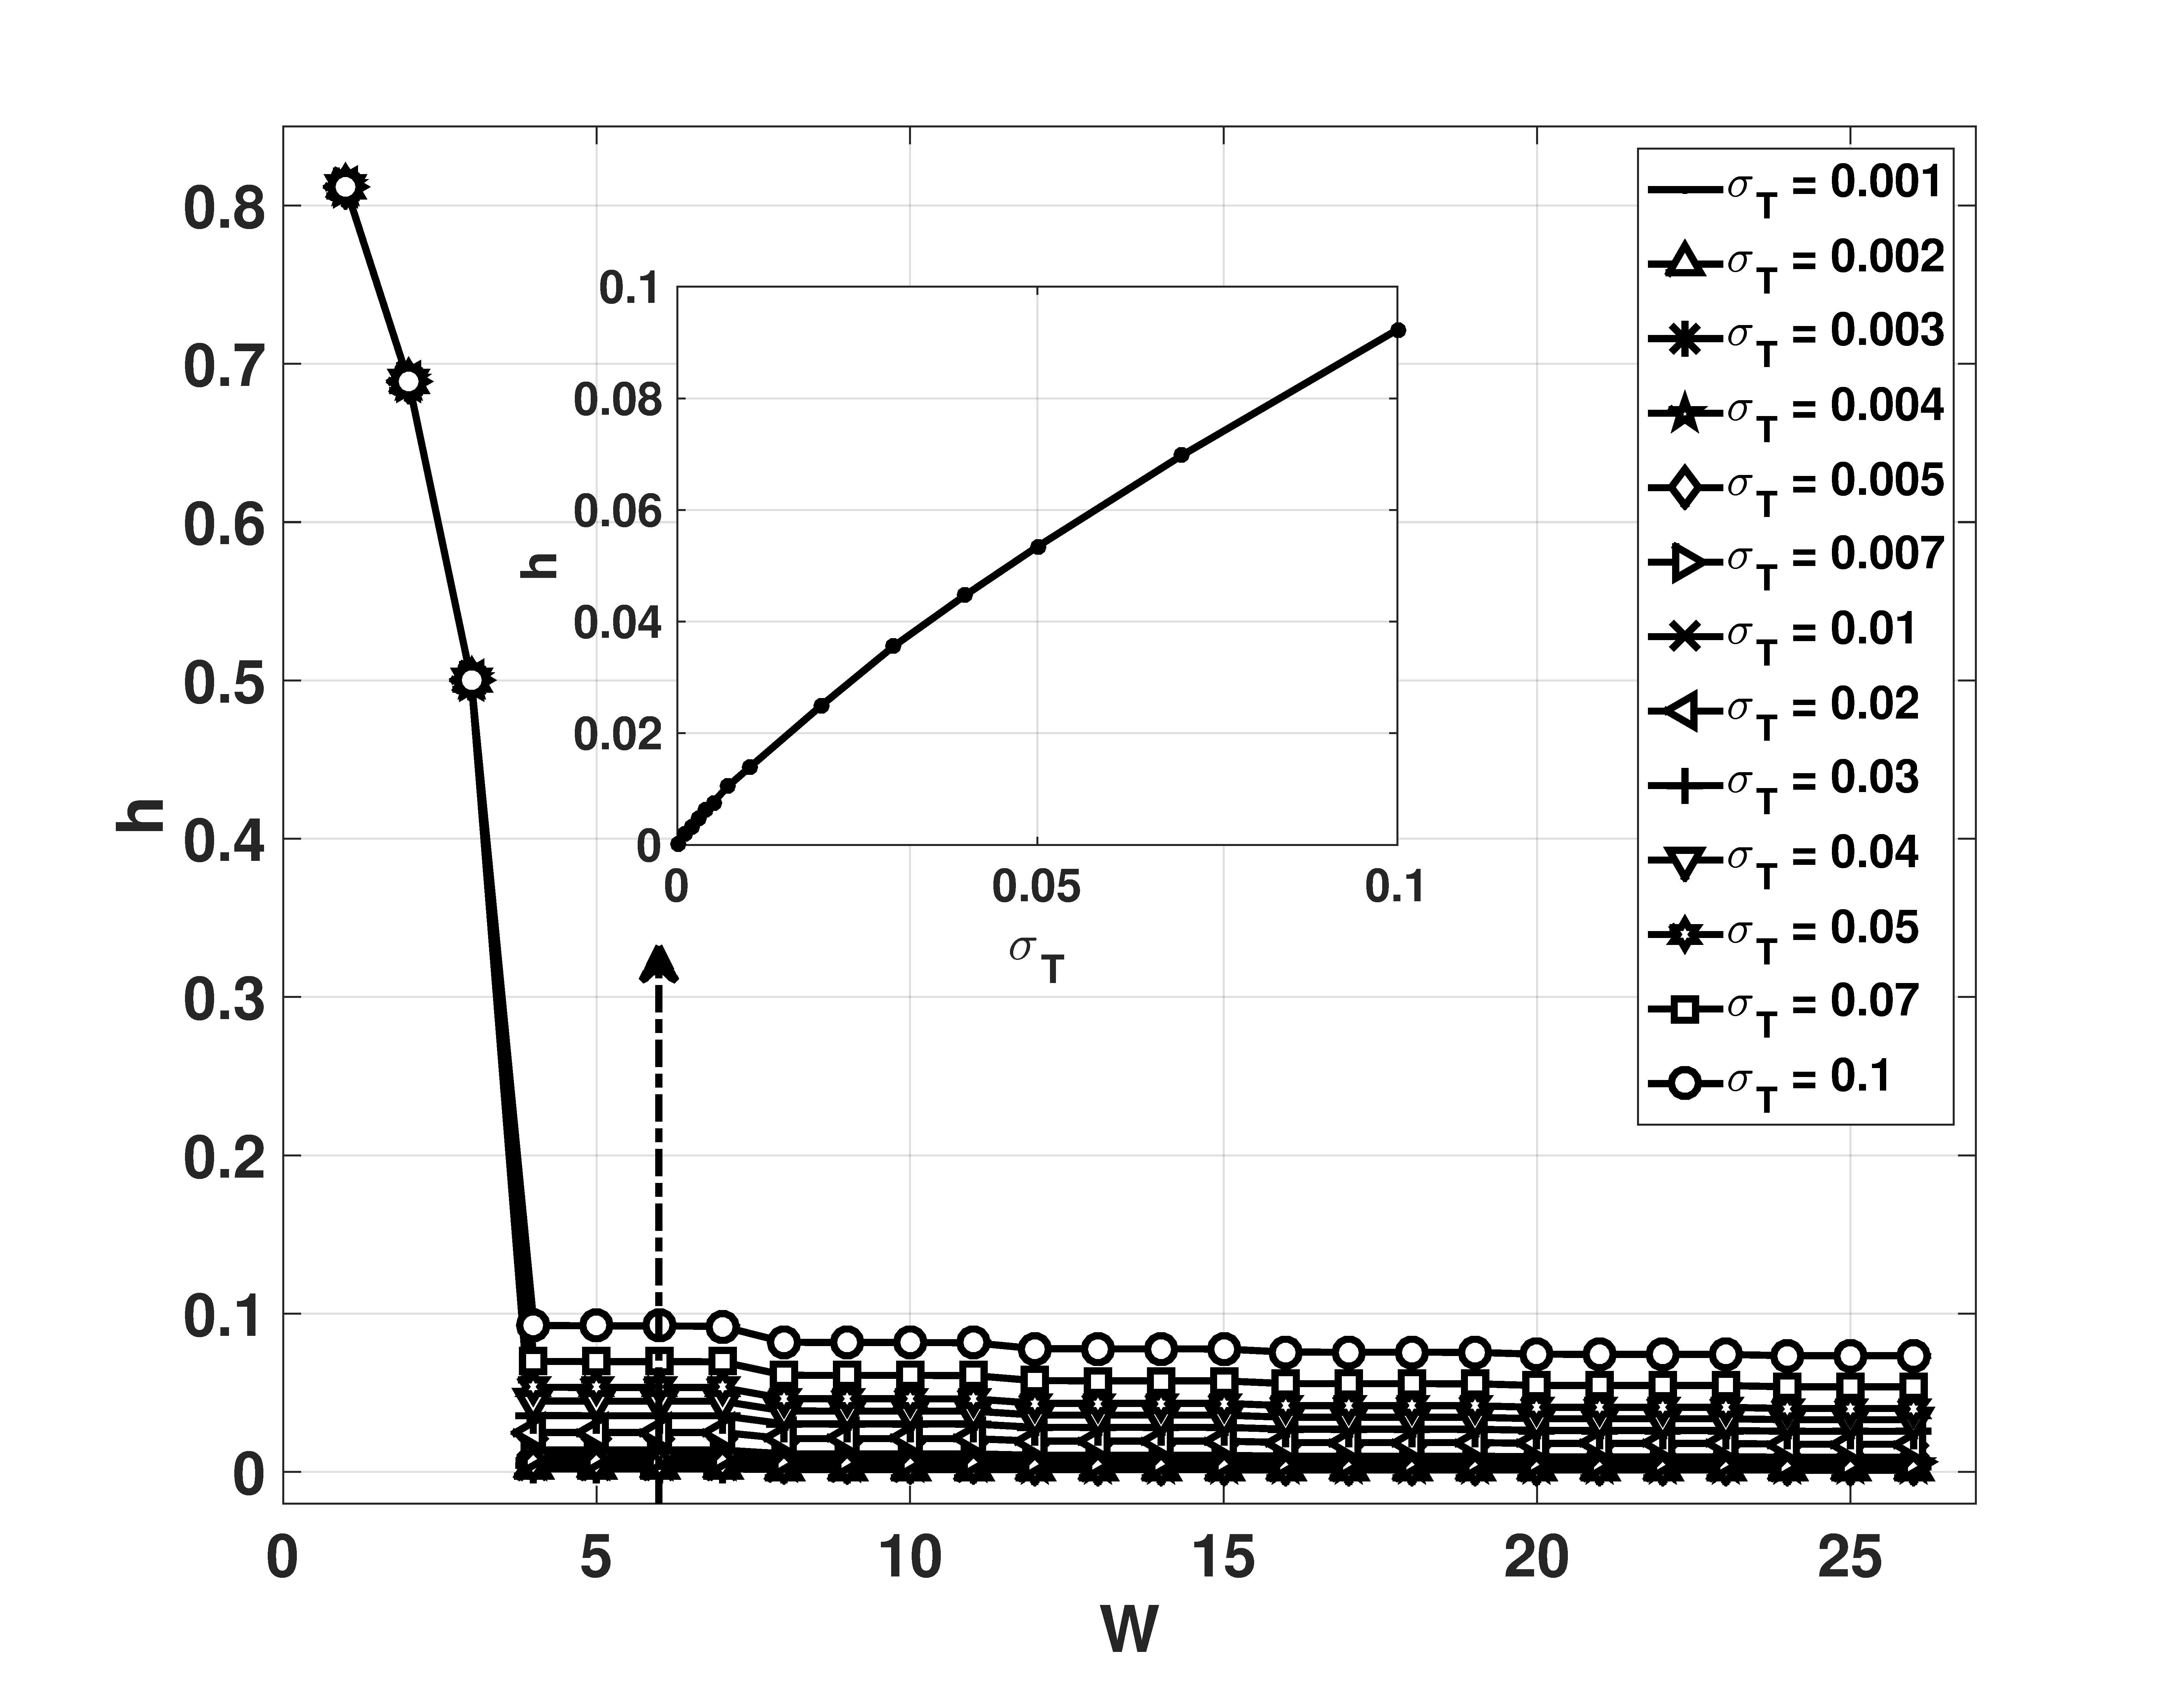
\includegraphics[ width=0.8\textwidth]{h_W_CJ}
\caption{$h$ en función de $W$ para un \emph{RO} muestreado con $r=8$, con \textit{jitter} con distintas varianzas. El recuadro muestra $h$ en función de $\sigma_T$ con $r=8$ y $W=6$.}
\label{fig:h_W_CJ}
\end{figure}

\begin{figure}
\center
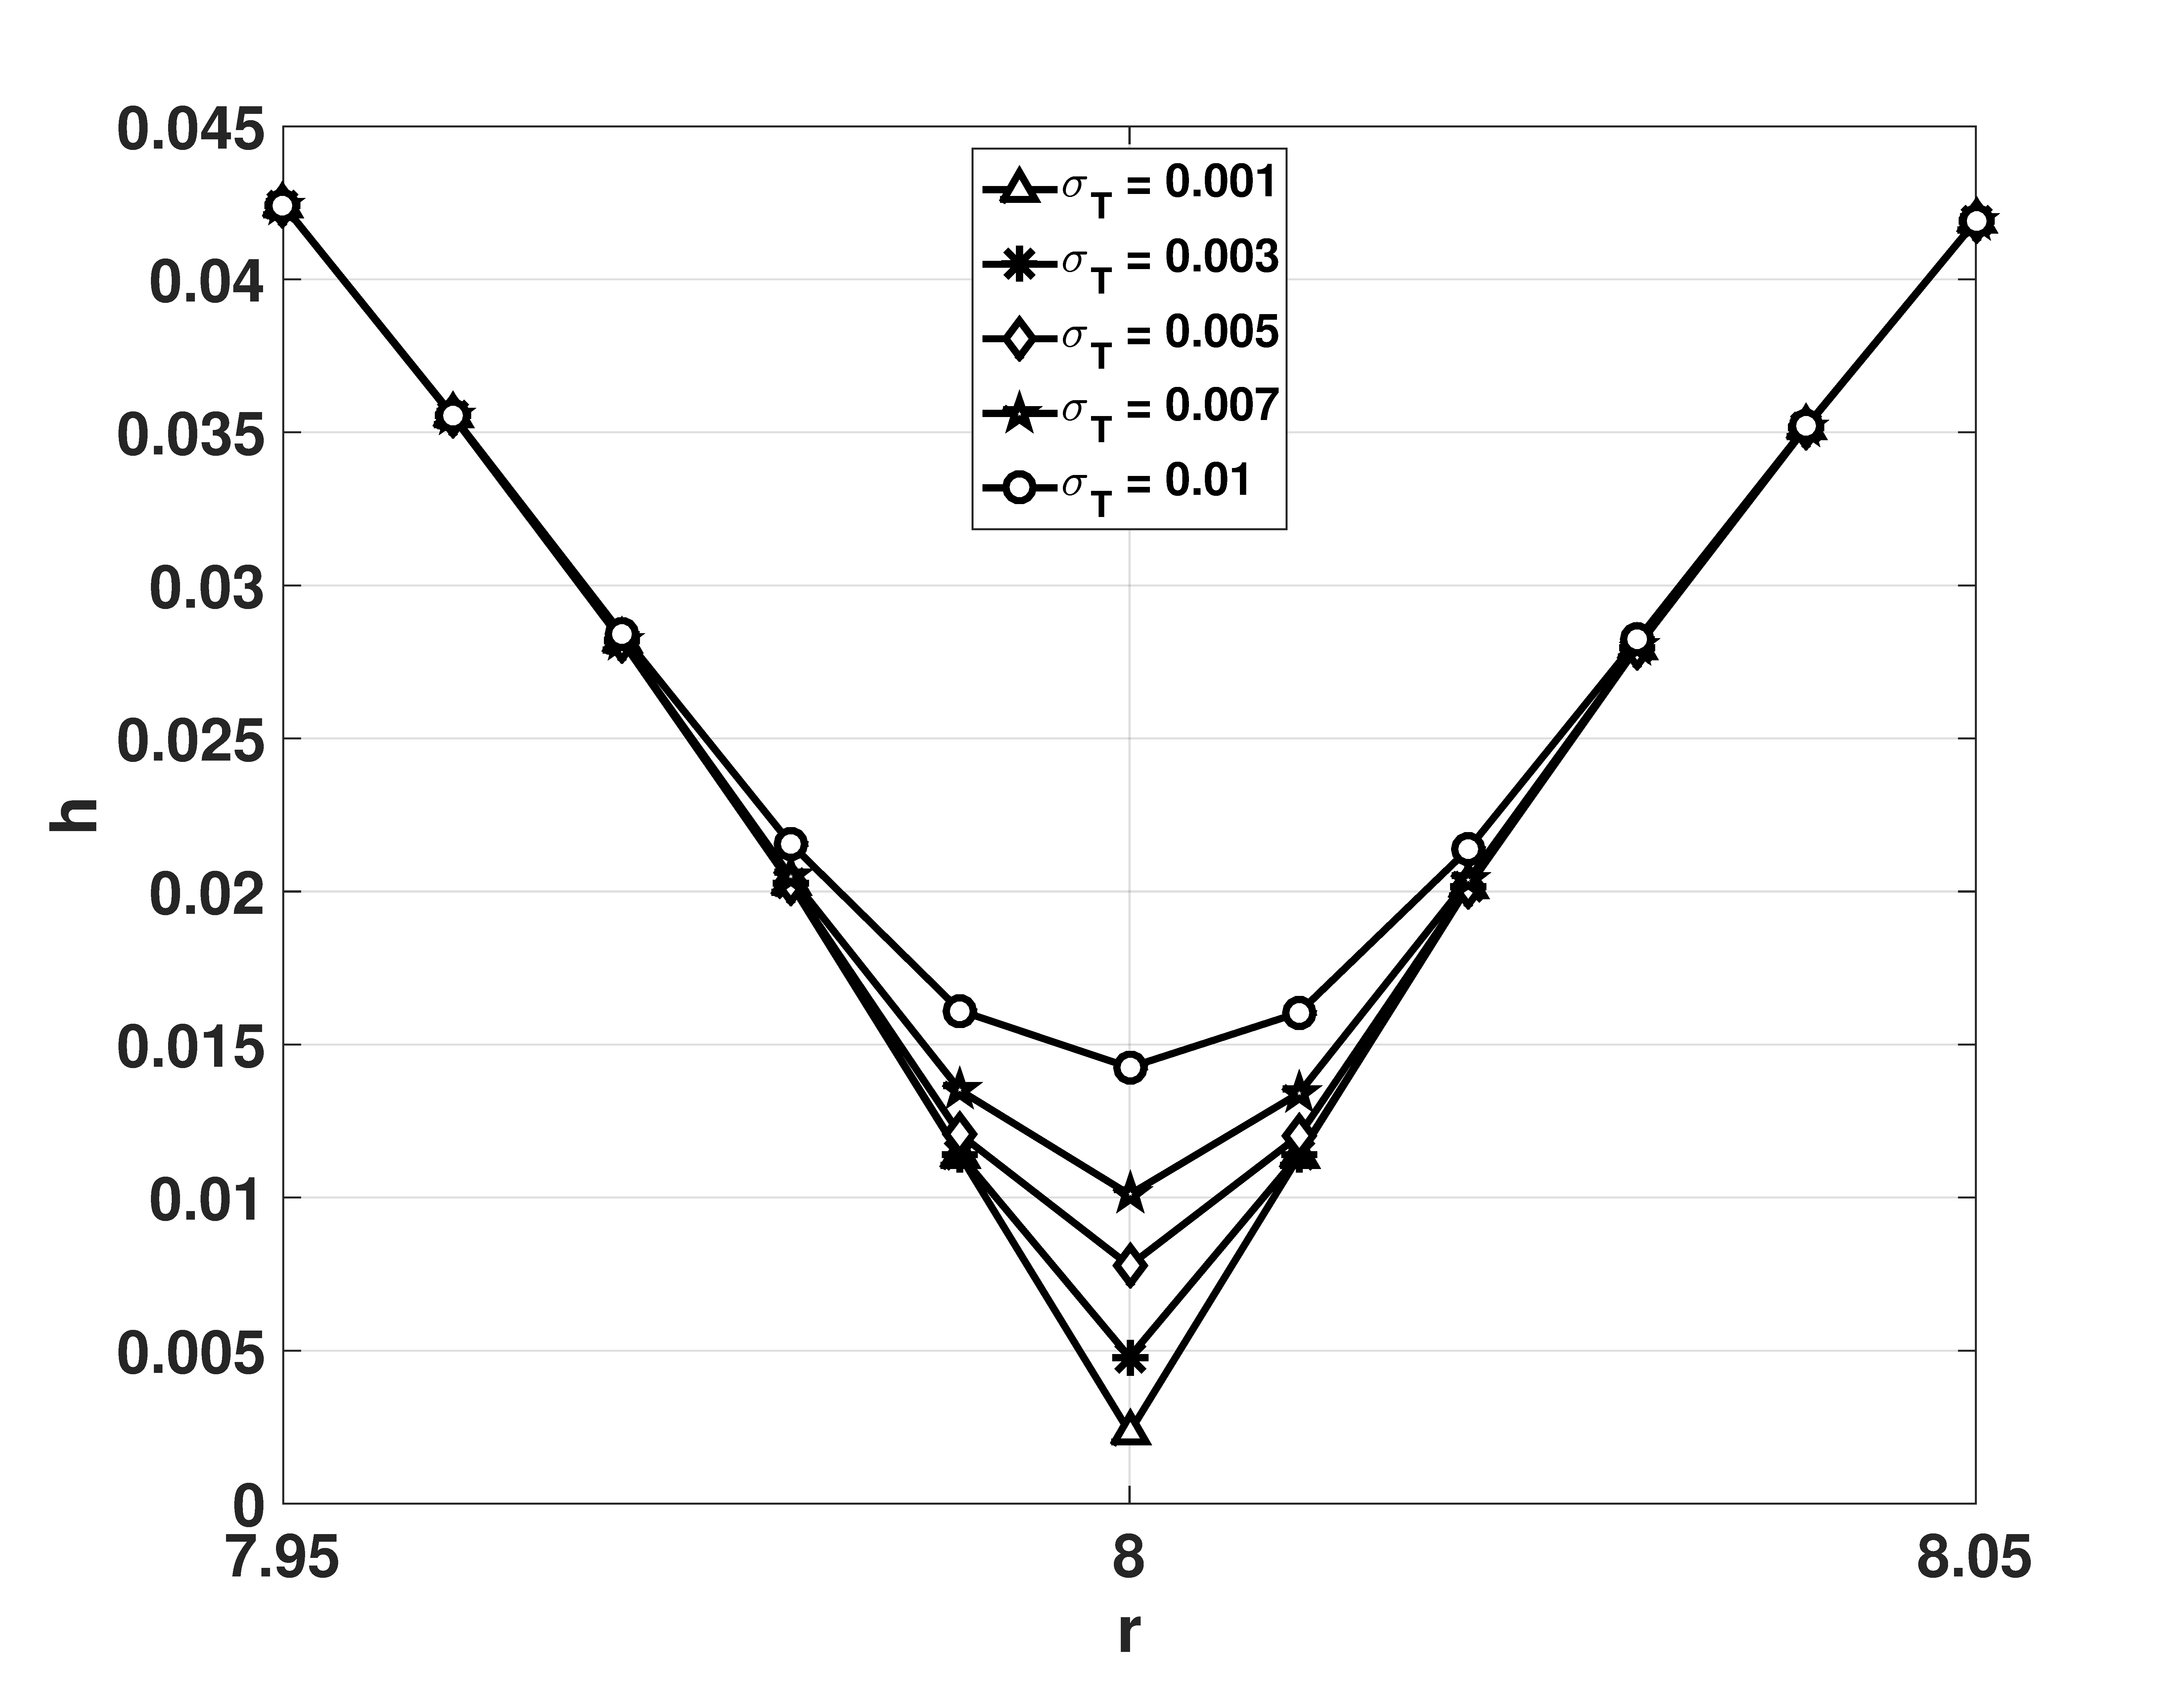
\includegraphics[ width=0.8\textwidth]{h_r_CJ}
\caption{$h$ en función de $r$ con $r\in[7.95,8.05]$, para distintos $\sigma_T$ y $W=6$ . La curva tiene un mínimo en $r=8$.}
\label{fig:h_r_CJ}
\end{figure}

Se debe realizar un análisis adicional para asegurar que los valores seleccionados $W = 6$ y $D = 8$ produzcan archivos simbólicos con una buena estadística. Para un alfabeto dado $\mathcal{A}$ con $m$ elementos, y un archivo simbólico dado de longitud $n$, el parámetro de calidad $\alpha = n/m$, vea \ref{sec: quanti}.
La calidad es mejor a medida que $\alpha$ aumenta y se acepta un valor mínimo $\alpha = 10$.
De acuerdo con la sección \ref{sec: quanti} los valores seleccionados $W = 6$ y $D = 8$ proporcionan $\alpha_h \simeq 10^5$, $ \alpha_ {h^*} \simeq 175$ con superposición y $29$ sin superposición. Todos los casos dan $\alpha>10$ como es requerido.

%EN LA SECCIÓN CUANTI TENGO QUE PONER COMO SE CALCULA ALFA

Figure \ref{fig:hm_h_CJ} shows the $h^*_{m} \times h$ plane. The quantifiers have been calculated sweeping the values of $D$ from $2$ to $11$, and $W$ from $2$ to $26$ (both for $h^*$ and only $W$ in the case of $h_{hist}$).
Better differentiation is obtained for higher values of the parameters, this is because both quantifiers tend to quantify the source value for $D$ and $W$ equal to infinite.
Nevertheless, this is impossible in real practice, also the amount of data available limits the values of the parameters based to achieve good statistics. Therefore, we seek the minimum values (threshold value) of the parameters that discern the jitter good enough. In Figure \ref{fig:hvsh_8} it can be seen that for values of $W$ equal to $3$ or lower the $h_{hist}$ quantifier is insensitive to the variations of the jitter. Therefore, $W$ should be $4$ or higher, this result is in concordance with the threshold determined in Figures \ref{fig:hhistvsW_T8_CJ}. In the case of $h^*$ the $W$ value should be equal or higher than $4$ and the value of $D$ higher than $7$, again this result is in concordance with the ones derived from Figures \ref{fig:hmvsD_T8} and \ref{fig:hmvsD_CJ_T8}. The bottom left area of the plane is the one with better performance of both quantifiers.

La figura \ref{fig: hm_h_CJ} muestra el plano $h^*_{m} \times h$.
Los cuantificadores se calcularon barriendo los valores de $D$ de $2$ a $11$ y $W$ de $2$ a $26$ (barrimos ambos para $h^*$ y solo $W$ en el caso de $h_{hist}$).
Se obtiene una mejor diferenciación para valores más altos de los parámetros, esto es porque ambos cuantificadores tienden a cuantificar la entropía de la fuente cuando $D$ y $W$ tienden a infinito.
Sin embargo esto es imposible en la práctica real, la cantidad de datos disponibles limita los valores de los parámetros para lograr buenas estadísticas.
Por lo tanto, buscamos los valores mínimos (valor umbral) de los parámetros que distinguen el \textit{jitter} lo suficientemente bien.
En la figura \ref{fig:hvsh_8} se puede ver que para valores de $W$ iguales o menores a $3$, el cuantificador $h_{hist}$ no es sensible a las variaciones del \textit{jitter}.
Por lo tanto, $W$ debe ser $ $ o superior, este resultado está en concordancia con el umbral determinado en las Figuras \ref{fig: hhistvsW_T8_CJ}.
En el caso de $h^*$ el valor de $W$ debe ser igual o superior a $4$ y el valor de $D$ superior a $7$, nuevamente este resultado está en concordancia con los derivados de las Figuras \ref{fig : hmvsD_T8} y \ref{fig: hmvsD_CJ_T8}.
El área inferior izquierda del plano es la que tiene un mejor rendimiento de ambos cuantificadores, sin embargo es la que precisa un mayor esfuerzo de cómputo y una mejor estadística.

%TENGO QUE PONER EL PLANO EN LAS FIGURAS

Una comparación entre ambos cuantificadores se muestra en la figura \ref{fig:hm_h_CJ}.
Los marcadores corresponden a varianzas $\sigma_T=\{0,$ $0.001,$ $0.002,$ $0.003,$ $0.004,$ $0.005,$ $0.007,$ $0.01,$ $0.02,$ $0.03,$ $0.04,$ $0.05,$ $0.07,$ $0.1\}$.
Hay que tener en cuenta que la pendiente de cualquiera de estas curvas es $dh^*/dh$ y es igual al cociente entre pendientes de curvas en las inserciones de las Figs. \ref{fig: hm_D_CJ}, y \ref{fig: h_W_CJ}.
Si $dh^*/dh\to1$, $h^*$ es más sensible que $h$ para medir el \textit{jitter}.
La pendiente aumenta levemente de $\sim2.47$ para $W =5 $ a $\sim5.54$ para $W = 19$, esto muestra que $h^*$ se vuelve más sensible a medida que aumenta $W$.
	
\begin{figure}
\center
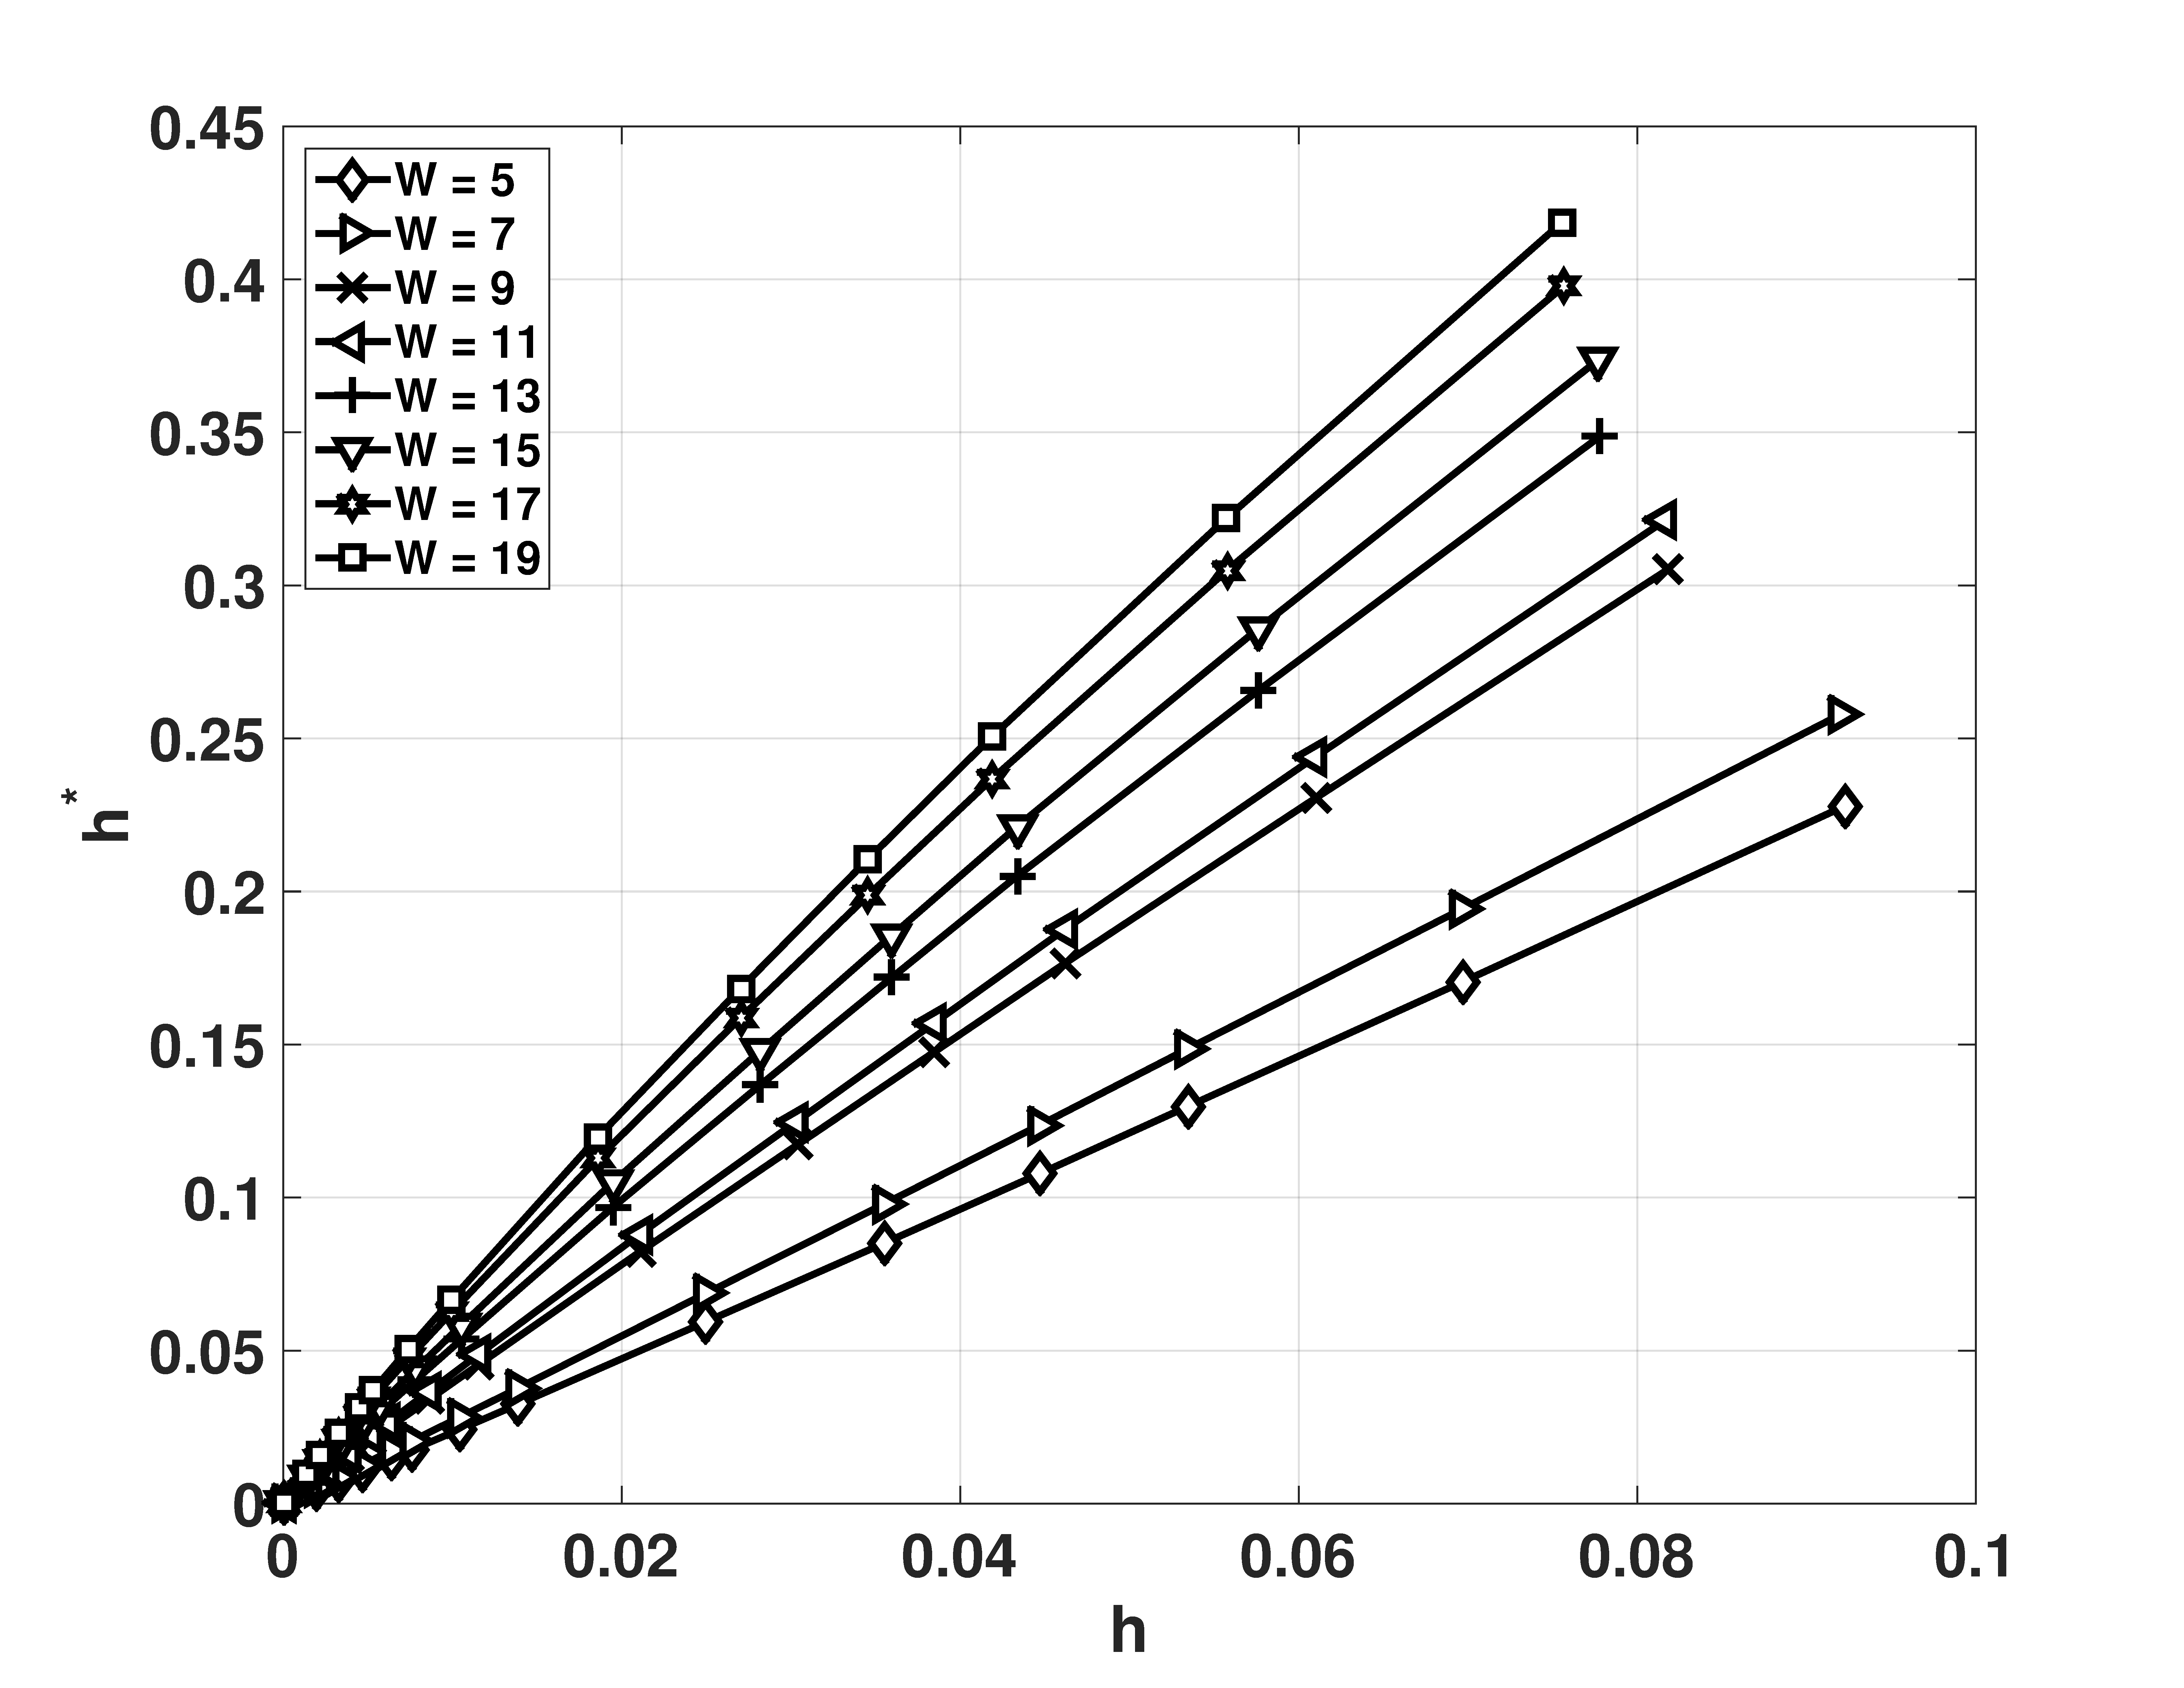
\includegraphics[ width=0.8\textwidth]{hm_h_CJ}
\caption{$h^*$ as a function of $h$ for $r=8$, $D=8$ and different values of $W$.}
\label{fig:hm_h_CJ}
\end{figure}

También evaluamos $h^*$ sin la superposición de bits entre números naturales consecutivos pero manteniendo la superposición de los $D-1$ números naturales entre patrones de orden (en todos los casos $h$ se evaluó con la superposición de $W-1$ bits consecutivos).
Los resultados se representan en la Fig. \ref{fig: Deltahm_Deltah_CS_SS} donde se muestra que al eliminar la superposición aumenta la sensibilidad de este cuantificador.
Por supuesto, obtenemos una cantidad menor de $W$ bits en números naturales del archivo original de siete millones de binarios, y en consecuencia, la calidad estadística es menor que la del cálculo original con superposición.
Para aumentar $\alpha$ hasta su valor anterior, se requieren archivos binarios más largos.

\begin{figure}
\center
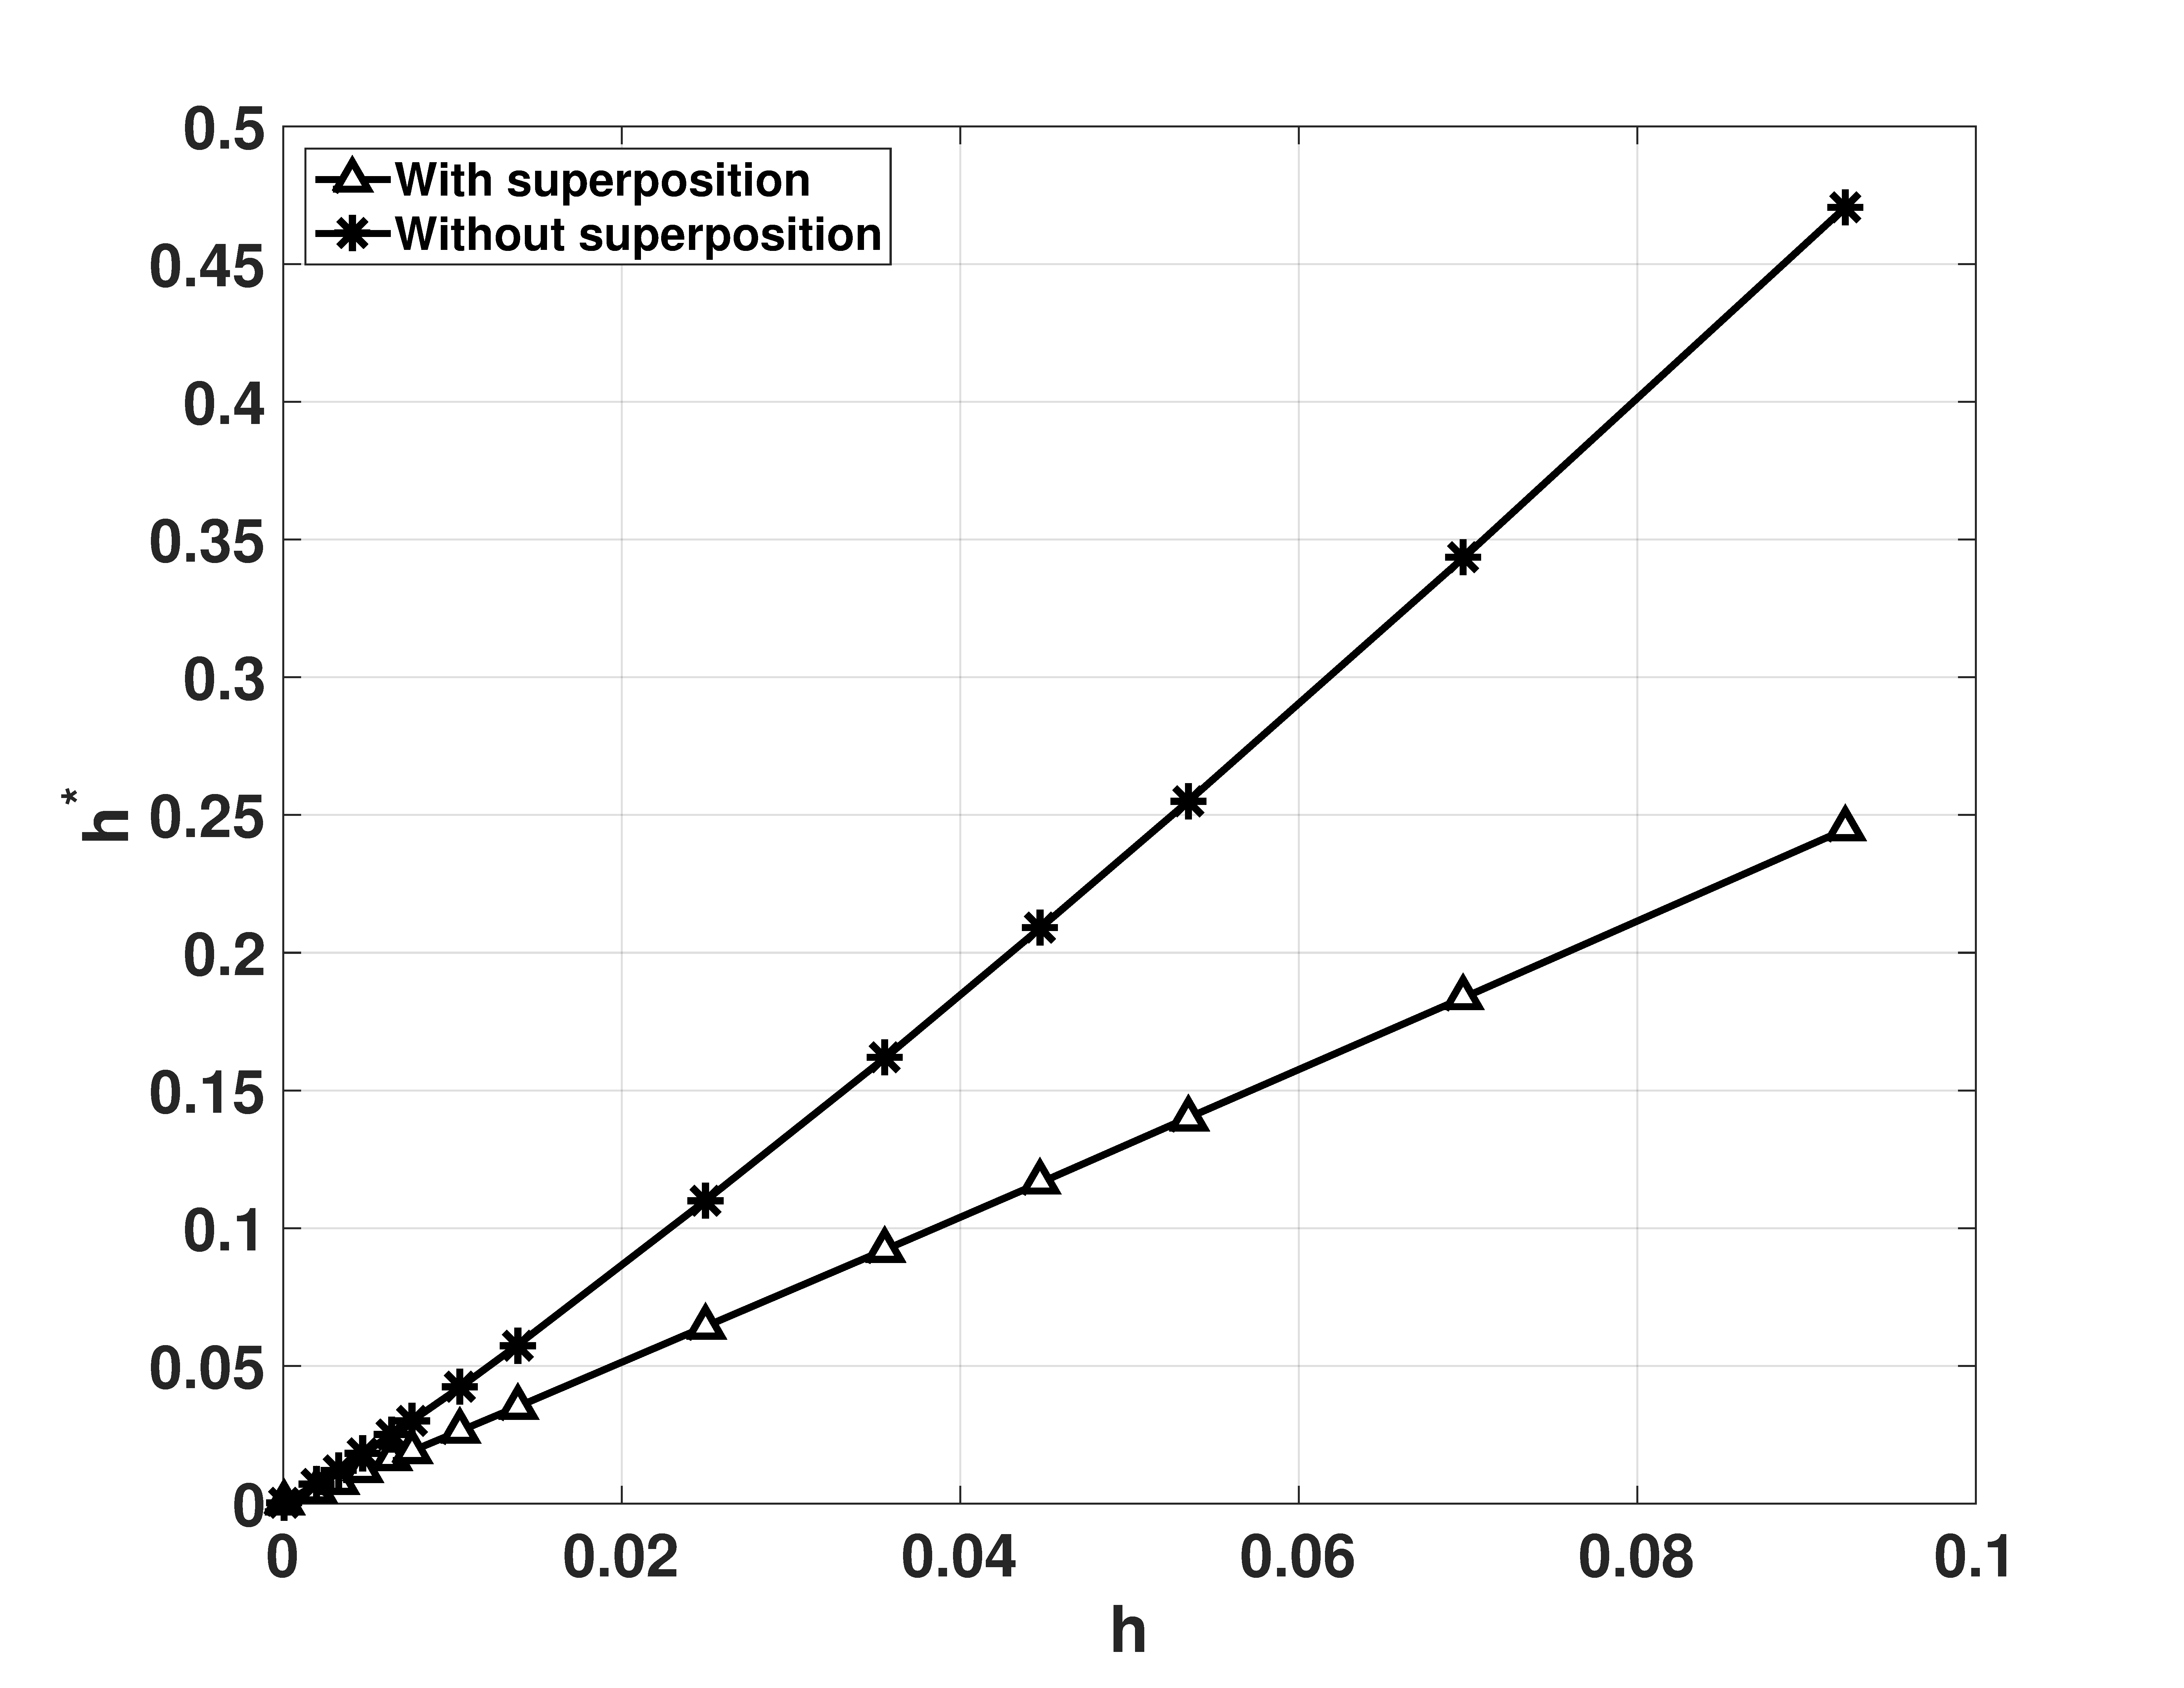
\includegraphics[ width=0.8\textwidth]{Deltahm_Deltah_CS_SS}
\caption{$h^*$ as a function of $h$ for $r=8$, $W=6$ and $D=8$. Two procedures to obtain $W$-bits natural numbers are considered: with and without superposition (see text).}
\label{fig:Deltahm_Deltah_CS_SS}
\end{figure}